%%%%%%%%%%%%%%%%%%%%%%%%%%%%%%%%%%%%%%%%%%%%%%%%%%%%%%%%%%%%%%%%%%%%%%%%%%%%%
%%% LaTeX-Rahmen fuer das Erstellen von Bachelorarbeiten
%%%%%%%%%%%%%%%%%%%%%%%%%%%%%%%%%%%%%%%%%%%%%%%%%%%%%%%%%%%%%%%%%%%%%%%%%%%%%

%%%%%%%%%%%%%%%%%%%%%%%%%%%%%%%%%%%%%%%%%%%%%%%%%%%%%%%%%%%%%%%%%%%%%%%%%%%%%
%%% allgemeine Einstellungen
%%%%%%%%%%%%%%%%%%%%%%%%%%%%%%%%%%%%%%%%%%%%%%%%%%%%%%%%%%%%%%%%%%%%%%%%%%%%%

\documentclass[twoside,12pt,a4paper]{report}
%\usepackage{reportpage}
\usepackage{amsmath,amsfonts,amssymb,amsthm}
\usepackage{mathtools}
\usepackage{commath}
\usepackage{svg}
\usepackage{textcomp} % degree
\usepackage{sidecap} %seitliche captions
\usepackage{apacite}
\usepackage{graphics, graphicx}
\usepackage{subcaption, framed, tcolorbox}
\usepackage[utf8]{inputenc}
\usepackage{latexsym}
\usepackage{todonotes}
\usepackage[margin=10pt,font=small,labelfont=bf]{caption}



\textwidth 14cm
\textheight 22cm
\topmargin 0.0cm
\evensidemargin 1cm
\oddsidemargin 1cm
%\footskip 2cm
\parskip0.5explus0.1exminus0.1ex
\setlength{\parindent}{7mm}

\pagestyle{headings}

\sloppy

\begin{document}

%%%%%%%%%%%%%%%%%%%%%%%%%%%%%%%%%%%%%%%%%%%%%%%%%%%%%%%%%%%%%%%%%%%%%%%%%%%%
%%% hier steht die neue Titelseite 
%%%%%%%%%%%%%%%%%%%%%%%%%%%%%%%%%%%%%%%%%%%%%%%%%%%%%%%%%%%%%%%%%%%%%%%%%%%%
 
\begin{titlepage}
 \begin{center}
  {\LARGE University of T\"ubingen}\\
  {\large Faculty of Science \\
Departement of Biology\\
Cognitive Neuroscience \\[4cm]}
  {\huge Bachelorthesis in Cognitive Science\\[2cm]}
  {\Large\bf  Exocentric Pointing in Virtual Reality: \large{Measuring the Intrinsic Geometry of the Visual Space} \\[1.5cm]}
 {\large Rahel Gerrens}\\[0.5cm]
\today\\[3cm]
\begin{center}{\small\bf Supervisor}\\[0.5cm]
{\large Prof. Dr. Hanspeter A. Mallot}\\
  {\footnotesize Cognitive Neuroscience, Faculty of Science\\
	University of T\"ubingen}	\end{center}
	
	
  \end{center}
\end{titlepage}

%%%%%%%%%%%%%%%%%%%%%%%%%%%%%%%%%%%%%%%%%%%%%%%%%%%%%%%%%%%%%%%%%%%%%%%%%%%%
%%% Titelr"uckseite: Bibliographische Angaben
%%%%%%%%%%%%%%%%%%%%%%%%%%%%%%%%%%%%%%%%%%%%%%%%%%%%%%%%%%%%%%%%%%%%%%%%%%%%

\thispagestyle{empty}
\vspace*{\fill}
\begin{minipage}{13.2cm}
\textbf{Gerrens, Rahel:}\\
Exocentric Pointing in Virtual Reality: Measuring the Intrinsic Geometry of the Visual Space\\ 
Bachelorthesis in Cognitive Science\\
Eberhard Karls University of T\"ubingen\\
Processing period: 28.05.2020-28.10.2020
\end{minipage}
\newpage

%%%%%%%%%%%%%%%%%%%%%%%%%%%%%%%%%%%%%%%%%%%%%%%%%%%%%%%%%%%%%%%%%%%%%%%%%%%%

\pagenumbering{roman}
\setcounter{page}{1}

%%%%%%%%%%%%%%%%%%%%%%%%%%%%%%%%%%%%%%%%%%%%%%%%%%%%%%%%%%%%%%%%%%%%%%%%%%%%
%%% Seite I: Zusammenfassug, Danksagung
%%%%%%%%%%%%%%%%%%%%%%%%%%%%%%%%%%%%%%%%%%%%%%%%%%%%%%%%%%%%%%%%%%%%%%%%%%%%
\section*{Zusammenfassung}
Luneburg nahm in 1947 infolge einer theoretischen Analyse an, dass die intrinsische Geometrie des visuellen Raumes konstant hyperbolisch gekrümmt ist. Diese Hypothese wurde vielfach getestet, so auch von Koenderink, van Doorn und Lappin (2000), indem sie die Krümmung der horizontalen Ebene vor den Augen untersuchten. Sie verwendeten die neue Methode des exocentric pointing,
bei der sich der Pointer, das Target und der*die Proband*in alle an unterschiedlichen Positionen befinden, und maßen die Win\-kel\-ab\-wei\-chung. Ihre Ergebnise zeigen im Gegensatz zu Luneburg eine nicht-konstante Krümmung des visuellen Raumes, die von der Distanz des*der Proband*in zu den Stimuli abhängt. Das folgende Experiment verwendete diese Methode des exocentric pointing von Koenderink et al. (2000), um den Einfluss der Beleuchtung (dunk\-le vs. helle Bedingung) und damit den Einfluss weiterer Tiefeninformation auf die Winkelabweichung zu untersuchen. Weiterhin wurden die Faktoren des Winkels des Pointers relativ zu dem Target und dem*der Proband*in, der Abstand des*der Proband*in zu den Stimuli und der Seite, auf der der Pointer positioniert wurde, untersucht. Das Experiment wurde in einer virtuellen Umgebung in einem Modell eines Untersuchungsraumes durchgeführt. Unsere Ergebnisse zeigten wie auch die Studie von Koenderink et al. (2000) eine nicht-konstante Krümmung des visuellen Raumes, mit al\-ler\-dings gegenteiligen Ausprägungen: Der visuelle Raum war bei uns hyperbolisch im Nahen und elliptisch in der Ferne. Des Weiteren hatte die Beleuchtung einen großen Einfluss und bewirkte eine positivere Winkelabweichung in der dunklen Bedingung mit weniger Tiefeninformation. 

\newpage

\section*{Abstract}
Luneburg proposed in 1947 by theoretical analysis that the intrinsic geometry of the visual space is of constant hyperbolic curvature. Many tested this hypothesis including Koenderink, van Doorn, \& Lappin (2000) by examining the curvature of the horizontal plane in front of our eyes. They used the novel method of exocentric pointing, in which pointer, target and subject are all placed at different positions, and measured the angular deviation. Their results showed opposing Luneburg a non-constant curvature of the visual space dependent on the distance of the subject to the pointer and the target. Our experiment used this method of exocentric pointing of Koenderink et al. (2000) to test the influence of the lighting (dark vs. light condition) and therefore examined the influence of additional depth cues on the angular deviation. Other factors tested were the angle at which the pointer was standing relatively to the targets and the subject, the distance of the subject to the stimuli and the side the pointer was standing at. The experiment took place in a virtual reality model of a lab room. Our results show like Koenderink et al. (2000) %kommata für diese apposition
a non-constant curvature of the visual space, but with opposite curvatures: We found the visual space to be hyperbolic in near space and elliptic in far space. Furthermore the lighting had a strong influence with more positive deviations found in the dark condition with less depth cues. 
\newpage

\section*{Danksagung}
Vielen Dank an Prof. Dr. Hanspeter A. Mallot und den gesamten Lehrstuhl Kognitive Neurowissenschaft für die gute Betreuung und die Offenheit, meine Fragen zu beantworten. Dank an Laura Häge für die tolle Arbeitsatmosphäre und die viele gemeinsame Zeit im Büro. Dank an Carina Siedle, Laura Häge und Sarah Fetscher, die diese Arbeit Korrektur gelesen haben.
Und zu guter Letzt Dank an meine Familie, meine WG und mein gesamtes Umfeld, die sich geduldig immer wieder meine kleineren und größeren Schwierigkeiten mit dieser Arbeit angehört, ertragen und mich ermutigt haben.
%%%%%%%%%%%%%%%%%%%%%%%%%%%%%%%%%%%%%%%%%%%%%%%%%%%%%%%%%%%%%%%%%%%%%%%%%%%%%
%%% Inhaltsverzeichnis
%%%%%%%%%%%%%%%%%%%%%%%%%%%%%%%%%%%%%%%%%%%%%%%%%%%%%%%%%%%%%%%%%%%%%%%%%%%%%
\newpage
\renewcommand{\baselinestretch}{1.3}
\small\normalsize

\tableofcontents

\renewcommand{\baselinestretch}{1}
\small\normalsize

%%%%%%%%%%%%%%%%%%%%%%%%%%%%%%%%%%%%%%%%%%%%%%%%%%%%%%%%%%%%%%%%%%%%%%%%%%%%%
% Der Haupttext startet hier
%%%%%%%%%%%%%%%%%%%%%%%%%%%%%%%%%%%%%%%%%%%%%%%%%%%%%%%%%%%%%%%%%%%%%%%%%%%%%
\newpage
%\cleardoublepage
\pagenumbering{arabic}
\setcounter{page}{1}

%%%%%%%%%%%%%%%%%%%%%%%%%%%%%%%%%%%%%%%%%%%%%%%%%%%%%%%
%%%%%%%%%%%%%%%%% INTRODUCTION %%%%%%%%%%%%%%%%%%%%%%%%
%%%%%%%%%%%%%%%%%%%%%%%%%%%%%%%%%%%%%%%%%%%%%%%%%%%%%%%

\chapter{Introduction}
\label{Introduction}

%\subsection{Background Kant}
%In Kant's Prolegomena %or maybe somewhere else
%he calles Euclidean geometry as a priori. 
%Euclidean geometry is based on the five axioms, the fivth being the paralell axiom \cite{Coxeter.1998}.
%When Kant is calling a piece of information a priori, this means, this information must be  true. But as the fifth axiom is not necessarily given in non-Euclidean geometry geometry, Euclidean geometry cannot be a priori. This opens a wide discussion on to what extend Kant's further conclusions are all invalid. 
% Kants opinions
% non euclidean geometry would falsify what of Kants opinion 
\section{Euclidean and non-Euclidean geometry} 
When we see something, we expect it to be also found in the physical world. We have learnt that when we see something, physical interaction confirms us that it is actually found there. If one had to explain  the geometry of what we see, they would say that it is most likely an identical depiction of the actual world. Thus as we interact with our world, as if it was a Euclidean space, we would also expect our visual space to be Euclidean space.

Euclidean space is something we are very familiar with. In two dimensions it simply is a plane. For example on a map of a town we can describe the position of a building using coordinates. If we were to choose two distances on the map with the same length, they would represent the same physical distance. %helpfull?
For all two points one would choose on such a map the shortest path between the two points is always a straight. Euclid had five postulates for his geometry, the latest of which was later on called the axiom of parallelism: "There is at least one line $q$ and at least one point $A$, not on $q$, such that no more than one line can be drawn through $A$ coplanar but not meeting $q$" \cite[p.~186]{Coxeter.1998}.

Non-Euclidean geometry is something we are more seldomly confronted with in our everyday lives. Gauss was the first to make non-Euclidean space applicable \cite{Parrochia.2018}. In such a space the shortest path between two points is not necessarily a straight. He called the shortest path between two points a geodesic. On our map the geodesic between any two points would be a straight, but in a non-Euclidean space it is different. Imagining the shortest path between London and Beijing, one can easily understand a geodesic. As our earth is not flat, the space we are in is non-Euclidean and the shortest path between the two cities is a geodesic. As the earth is roughly a sphere the geodesic is a circular arc.  %mathematical definition of a geodesic Gauß-Bonnet Theorem? %more general on non-euclidean space?
% schreibweise: \non-euclidean, oder non-Euclidean, eher letzteres
In non-Euclidean space, the just mentioned parallel postulate is not given \cite{Coxeter.1998}. For example, for the longitudes of our earth, being elliptic, the parallelism of these lines is not given as they all merge at the poles.
Later on, Riemann generalised Gauss' idea to manifolds of three or more dimensions \cite{Luneburg.1947}.

\section{Binocular vision}
One has to differentiate between the visual space and the physical space. Luneburg \citeyear{Luneburg.1947} defines the visual space as the visual sensation of our surrounding, not only including the colours and brightness of the objects of our surrounding, but also their localisation in a three-dimensional space. This space has got a geometry, which is then called the intrinsic geometry of the visual space. It needs to be differentiated from the extrinsic geometry, which describes the relationship between the visual space and its surrounding space \cite{Fernandez.2009}. This surrounding space is another way of measuring our environment by taking its physical measurements, for example by measuring the physical distance between two objects. Luneburg calls this the physical space. Scarcely surprising, they are mainly the same; after all, the visual space is a depiction of the physical space. But in some aspects they differ:

By having two eyes, two separate viewpoints are provided when perceiving the physical world. They allow binocular vision as two partially distinct images get transmitted, each by one eye. Our eyes have a common reference point called the egocenter, %was nützt diese Information?
located midway of the interocular axis, the axis between the two eyes \cite{DeValois.2000}. This allows the visual points of the two eyes to be mapped into one binocular space.
The result is then the one continuous image we call the seen image. 

There are visual points which are mapped onto the same position in both eyes. The horopter describes a group of such points. It is called horizontal horopter or frontal plane horopter, when examining the visual points on the horizontal plane in front of the eyes. One must distinguish between the theoretical and the empirical horopter. The theoretical horopter consists of the points furthest away from the eyes, which are mapped on corresponding positions on the retina. Hence the disparity of the two eyes at those points equals zero. Those are the points which are seen most easily \cite{DeValois.2000, Helmholtz.1867}. % ist dieser letzte satz hilfreich? berufts sich Helmholtz irgendwann auf diese Leichtigkeit?
They all align on a circular arc. The circle, they partly align on, is called a Vieth-Müller circle (see figure \ref{horopterLuneburg}).
\begin{figure}
    \centering
    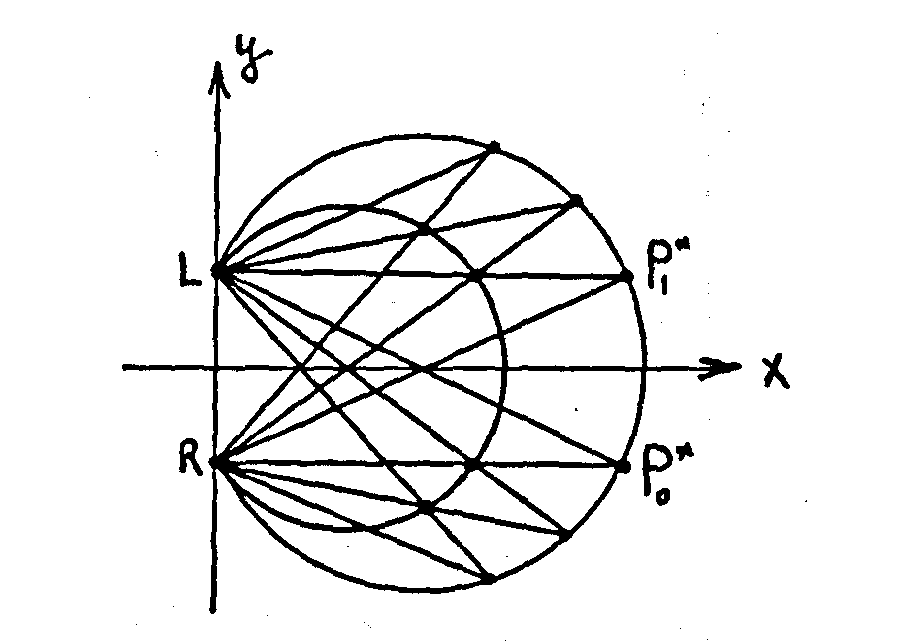
\includegraphics[width=7cm]{Images/Horopter from Luneburg 1950.png}%picture?
    \caption{The theoretical horopter. The points with zero disparity on both eyes are all found on the Vieth-Müller circle. L and R indicate left and right eye respectively. Taken from Luneburg (1950).} 
    \label{horopterLuneburg}
\end{figure}
The empirical horopter, on the other hand, is based on psychophysical observations, not on calculations, and differs from the Vieth-Müller circle. Its curvature can be steeper or flatter than the Vieth-Müller circle and it can be skewed \cite{DeValois.2000}.

The retinal image is only a two dimensional image lacking the third dimension, the depth dimension. Our brain reconstructs this dimension using different depth cues. 
Firstly, there is the stereopsis: the matching of the two retinal images allows depth perception, by using the binocular disparity \cite{Mallot.2000}. 
Other cues are lighting, hard shadow, at larger distances o\-pa\-ci\-ty, one object covering the other and the relative size of an object if the actual size is known. All these cues are based on experience \cite{Helmholtz.1867}.


\section{Luneburg's depth theory}
The basis for the depth theory is the geometrical analysis of binocular vision \cite{Helmholtz.1867, Luneburg.1947}. It is a purely mathematical analysis of binocular vision. Luneburg \citeyear{Luneburg.1950} himself said that his theory is no general theory of space perception as no psychological factors were included.
Von Helmholtz \citeyear{Helmholtz.1867} noticed that the visual space had a curvature. He placed 
three strings vertically next to each other on one plane. When looking at the strings, while the median plane of his face was cutting the middle string, the middle string appeared to be closer to him than the others. This effect increased by decreasing distance to the strings and even changed into the opposite at far distances (see figure \ref{empHoropterHelmholtz}). 
\begin{figure}
    \centering
    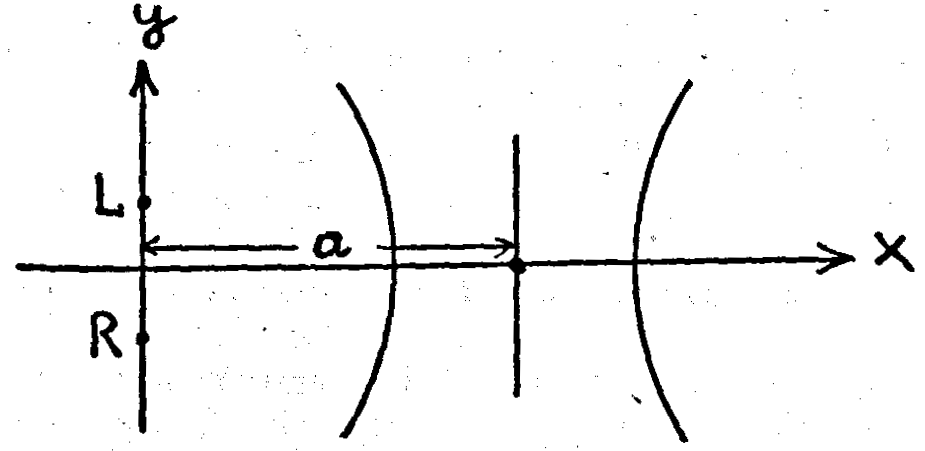
\includegraphics[width=7cm]{Images/HelmholtzEmpHoropter.png}%picture?
    \caption{Different empirical horopter curves for different fixations found by Helmholtz (1867). L and R indicate left and right eye respectively. Taken from Luneburg (1950).} %nicht optimal
    \label{empHoropterHelmholtz}
\end{figure}
%ref picture Luneburg
He concluded the visual space to be elliptic in near space. The extent of the effect, represented with $a$ in figure \ref{empHoropterHelmholtz}, was dependent on the person.
%to be elaborated

Luneburg went even further. He proposed the visual space to be of constant Gaussian curvature and derived a metric to translate from the physical space to the visual space. His hypothesis \citeyear{Luneburg.1947} was that the visual space is an integration of the information provided by the mathematical relation of the apparent size to the physical qualities of localisation and arbitrary parameters depending on the observer. %overkill
It depends on the physical position of the object, expressed in bipolar differentials, and depends on the localisation of the line element as one characterisation of the visual space. 
% ab hier möglicherweise streichen §§§§
The line element $ds$ can be represented by 
\begin{flalign}
ds^2 = dp^2 + \textnormal{sin}_K(\rho )^2 d\theta^2
\end{flalign}
where $\rho$ and $\theta$ are polar coordinates with $\rho$ denoting the perceived egocentric distance and $\theta$ denoting the perceived direction \cite{Heller.1997}. The function of $\textnormal{sin}_K(\rho)$ depends on $K$, i.e. if it is equal to zero, positive or negative. 
% bis hier §§§§
Luneburg assumes the value of $K$, denoting the Gaussian curvature, to be constant at any point in the visual space. The visual space is hyperbolic for $K > 0$, elliptic for $K < 0$ and Euclidean for $K = 0$.
He describes the curvature $K$ by 
\begin{flalign}
K = -e ^{-2\sigma \mu}
\end{flalign} where $\sigma$ and $\mu$ are constants. To determine these constants he leaves as a future research question \cite{Luneburg.1947}. He concludes the visual space to have a non-Euclidean geometry and conjectures it to be hyperbolic. He sees this confirmed  by observations of several authors, for example those of Blumenfeld in his alley experiments \cite{Blumenfeld.1913}, or those of von Helmholtz in his frontal horopter plane experiments \cite{Helmholtz.1867}.   

The necessity of the intrinsic curvature to be constant is controversial. %(Busemann, Freudenthal, Suppes) siehe Indow
Luneburg himself brought forth several arguments for a constant curvature \cite{Luneburg.1950}. If the metric space the distance function is defined on is homogeneous, the Riemannian space is of constant curvature. In empirical experiments a lack of absolute localisation was noticed and incorporating this principle into the psychometric distance function, this leads according to Luneburg to a homogeneous space. Secondly, as the appearance of the phy\-si\-cal object does not change when the object moves in the visual space, a constant curvature was assumed. This is related to the Helmoltz-Lie problem, %mäh
which discusses the conditions under which a physical object does not change size and shape when changing position \cite{Freudenthal.1965}. The solution is that physical space must be structured according to one of these geometries: $K = 0, K > 0, \textrm{or } K < 0$. Transferring this to the visual space, the visual space should be of constant curvature \cite{Indow.1991, Indow.1997}. On the other hand, some counter evidence to a constant curvature has already been found in experiments
\cite{Cuijpers.2001}.
%Gegenpositionen

One measure of the Gaussian curvature is given by the Gauss-Bonnet theorem.
Following this theorem, the total curvature of a polygon is measured by the angular excess \cite{wilson.2007}. For example, in a triangle in Euclidean space all angles add up to 180\textdegree{} \cite{Parrochia.2018}. 
The angular excess is hence the difference of the sum of the triangle's angles in non-Euclidean space to the angles' sum in Euclidean space. 
% absatz passt da eigentlich nicht rein. 
\section{Previous experiments}
Some have already tested Luneburg's hypothesis of the visual space being of constant curvature using different methods. The frontal plane horopter ex\-pe\-ri\-ment is based on the three-strings ex\-pe\-ri\-ment of Helmholtz \cite{Helmholtz.1867}. In the frontal plane horopter experiment subjects were asked to align several stimuli next to each other against a uniform background until they perceived them to be on a straight line. %discrimination of distant alley and parallel alley experiment?
In the alley experiment the subject also had to place stimuli on their eyes' horizontal plane, this time not parallel to their interocular axis but orthogonal \cite{Blumenfeld.1913}. At the far end two lights were fixed, the others had to be placed in two lines, so that the subject perceived them to be parallel. These experiments were usually conducted under non-natural conditions. They took place in the dark with only the lights being visible. The subjects' heads are placed on a headrest, hence only eye movement is possible. Thus in such an experiment only binocular disparity can be used as a depth cue. 

Zajaczkowska \citeyear{Zajackowska1956.} conducted both a frontal plane horopter experiment and alley experiments. He constructed three differerent alley experiments: the classic alleys, the intermediate alleys and the broad alleys, in which he varied increasingly the distance in between the furthest points. For his experiments he used Luneberg's formulas \cite{Luneburg.1950} to predict his results and to compare them with his own empirical data. The results of the frontal plane horopter experiment were close to the predictions. For subjects with a low absolute value of $K$ and good depth perception the measured and expected horopter differed less. The values of $\sigma$ (the higher, the better the depth perception) and $K$ were closest to the predicted for the broad alley experiment \cite{Zajackowska1956.}. %was ist mit mu passiert? 
As the subjects with good depth perception gave good support for Luneburg's hypothesis, he concluded on a non-Euclidean, hyperbolic visual space. 

Koenderink, van Doorn and Lappin \citeyear{Koenderink.2000} were the first to introduce the method of exocentric pointing to measure the geometry of the visual space and to test Luneburg's theory. They criticised the conditions of the pre\-ce\-ding experiments since those experiments having stimulus reduction to lights with no body movements allowed including head fixation (from now on called minimalistic experiments) did not measure up with our natural perception. They ascribed the preceding results to these constraints. Indeed, earlier experiments, which took place in an open field or a room with reference points, did not show constant curvature \cite{Cuijpers.2001, Battro.1976}.

That is why Koenderink et al. conducted their experiment in the field and allowed body movement. Only the eye height and the location the subjects were positioned at were constrained. Additionally, in contrary to Luneburg's theory, they did not assume the visual space to be of constant curvature, they only assumed the space to be Riemannian and isotropic \cite{Koenderink.2000}. They claimed to be able to describe the intrinsic curvature as a function of distance, i.e they expected the curvature of the intrinsic visual space to be dependent on the distance of the subject to the perceived objects. 

Exocentric pointing needs to be differentiated from normal pointing or aiming, as the object one is pointing with is at a different position than oneself. Hence the subject, the pointer and the target are all at three different positions, forming the three corners of a triangle. The task of the subjects was fairly simple, as to point with the pointer at the target. The pointer was rotatable on its y-axis by the subject via a remote controller. The construction of Koenderink et al. \citeyear{Koenderink.2000} for the pointer allowed good recognition of the pointer's orientation. The pointer consisted not only of an arrow for pointing, but the arrow was spiking a cube. This had the advantage that, additionally to the length of the arrow $(\alpha/\bar \alpha)$, the size's relation of the cube's faces $\lambda / (\lambda -1)$ indicated the pointer's orientation (see figure \ref{figSchematicPointer}). 
\begin{figure}
    \centering
    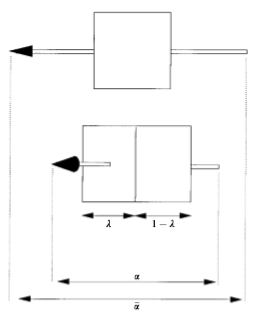
\includegraphics[width=6cm]{Images/PointerSkize.PNG}%picture?
    \caption{Schematic image of the pointer as it appears to the subject with relational sizes in the study of Koenderink et al. (2000).} %nicht optimal
    \label{figSchematicPointer}
\end{figure}

Their results showed a deviation from the veridical angle, hence also showed a curvature of the visual space. The deviation and therefore the intrinsic curvature depended on the distance of the subject to the target. Therefore Koenderink et al. \citeyear{Koenderink.2000} showed counter-evidence for Luneburg's hypothesis of constant intrinsic curvature. Their results suggested intrinsic visual space to be elliptic in near space and hyperbolic in far space.
%WHAT IS THIS STRANGE THING ABOUT -K AND STILL HYPERBOLIC SPACE?

\section{Aims of this study}%herleitung zum eigenen experiment
Our experiment is also going to try measuring the intrinsic geometry of the visual space by looking at possible deviations on the horizontal plane at eye height.
All preceding experimenters assumed the geodesics to be the best way to describe the curvature in their experiments. Even if a geodesic is a neat mathematical description of a curvature, it does not make the description necessarily more likely, especially if also the interference of other psychological factors is taken into account. Additionally, with the results of Koenderink et al. there are contradictory results concerning the constancy of the intrinsic visual space. Therefore our experiment is going to test Luneburg's hypothesis of a constant curvature again. It is going to use the method of exocentric pointing of Koenderink et al. \citeyear{Koenderink.2000}. 

Something that has not been considered enough so far is the influence of environmental cues on the depth perception. The surrounding may have a strong influence on the perceived depth; as described earlier, the environment provides many different depth cues. This may influence the deviation. In the minimalistic experiments this could have not been the case. That is why in our experiment there will be two conditions, one of which is a minimalistic experimental condition taking place in absolute darkness (in the following called dark condition), hence eliminating all environmental depth cues. The other one is conducted under natural illumination (in the following light condition). This comparison will allow us a first examination of that presumable environmental influence. 

%why virtual reality?
All preceding minimalistic experiments \cite{Zajackowska1956., Indow.1991} %(und co),
were conducted in lab rooms, which were darkened artificially. In many experiments today virtual reality glasses are used. They allow the stimuli to be more controlled. Using virtual reality glasses for the minimalistic experiments has many advantages. For example, absolute darkness can be guaranteed and all movement can be inhibited without a head rest. The subject may be absolute na\"{i}ve of the room structure and the targets' positions. Additionally, if using virtual reality is confirmed as a possible experimental set-up for exocentric pointing, this opens a wide range of possibilities: Stimuli, room or other cues can be tailored for the experiment without any restrictions \cite{Gaggioli.2001}. Those advantages need to be evaluated in relation to the drawbacks such as limited field of view or possible underestimation of distance \cite{Interrante.2008}.

\subsection{Hypotheses}
Parallel to this experiment another experiment took place with the same conditions, however not conducted in virtual reality, but in an actual lab room (in the following called real life experiment). We expect that our virtual reality experiment will provide similar results to the real life experiment.

Secondly, we expect the curvature not to be dependent on the side the pointer is standing at, i.e. we expect the curvature to be symmetrical in the dark condition, as in minimalistic experiments symmetry has already been shown \cite{Indow.1991}. In the light condition the symmetry could not be given as clearly as in the dark condition, as the surrounding environment not visible in the dark provides depth cues and thus may influence the perceived depth. These cues may be different when pointing into the opposite direction. 
If there is a difference between dark and light condition, the geodesics alone are possibly not sufficient to describe the intrinsic visual curvature. Then, interference of the structure of the room can be concluded.

Thirdly, our main hypothesis is that the deviation of the angle, i.e. the error the subjects are making, will depend on the angle of the pointer in relation to the target and the subject and will display no constant curvature. This angle is dependent on the subject position and the target position. As this is the first experiment having such a set-up, no more specific hypothesis to what extent the angle will change under which condition is reasonable. Still some predictions can be made: The smallest angles are found, when the distance between the subject and the pointer is the smallest, while the largest angles are found, when the distance between the subject and the pointer is the largest. Transferring the results of Koenderink et al. \citeyear{Koenderink.2000} and Zajaczkowska \citeyear{Zajackowska1956.} onto our experimental setting, even though the scale of the experimental setting is different, we would expect an undershoot for the smaller angles and an overshoot for the larger angles. %still not ideal last sentence


% von Helmholtz vs Helholtz

% explanations YangPurves explanation of probability. 

% Luneburg assumes symmetry (or his function). (631f)

% zeitform konstant perfect

%winkelsummer größer elliptisch, winkelsumme kleiner hyperbolisch

% in fig schematicAUfbau, subject positions need to be labelled 
% Zahlen ausschreiben?
\cleardoublepage
%%%%%%%%%%%%%%%%%%%%%%%%%%%%%%%%%%%%%%%%%%%%%%
%%%%%%%%%%%% Method %%%%%%%%%%%%%%%%%%%%%%%%%%
%%%%%%%%%%%%%%%%%%%%%%%%%%%%%%%%%%%%%%%%%%%%%%



\chapter{Method}
\label{Method}
Allowing the data to be comparable to the real life experiment, the experimental method imitated  the method of the real life experiment. 

\section{Participants}
Eight subjects participated. The first four had to be excluded due to erroneous experimental settings. All were students of the university of Tübingen, na\"{i}ve to the hypotheses. All subjects had normal or corrected sight. Their age ranged from 22 - 25 ($\mu = 22.75$, $SD = 1.50$), all were right handed, one was male, three female. 
%ist diese trennung der beiden Subjectgruppen sinnvoll?
Additionally to these subjects, one subject (21, right handed, female) was tested, which already had participated in the real life experiment. Obviously, this subject was not na\"{i}ve to the hypotheses, was familiar with the room structure and was more used to the experimental task.

\section{Apparatus}
For the presentation of the experiment, a HTC Vive Pro (HTC Corporation, 2011-2020) was used via a head mounted display (HMD). The HMD had a re\-so\-lu\-tion  of 1440 $\cdot$ 1600 pixels per eye (stereo vision), with an image rate of 90Hz and a 110\textdegree{} field of view. The virtual reality environment and the experimental set-up were created with the game engine Unity (version 2019.3.3f, Unity Technoligies 2020). For the calibration of the HMD and the controller, for the presentation and saving of data a SteamVR application program interface and the SteamVR Unity Plugin version 2.5 (Valve Corporation, 2020) were used. 

\section{Stimuli}
The composition of the experiment was similar to Koenderink et al. \citeyear{Koenderink.2000} using the method of exocentric pointing and using a similar composition of the pointer. A rotatable pointer placed on a tripod was utilised. It consisted of a cube with 20cm edge length, pierced with an "arrow", a rectangular bar of 1m length and an edge length of 3cm, sticking out 40cm at each side. In total, the apparatus of the pointer was 1.365m tall, with the arrow at a height of 1.25m. The arrow was coloured in yellow, the cube was coloured in pale orange, except for the cube's face facing towards the subject, which was coloured in yellow like the arrow. The  cube's faces  gave various monocular cues for the rotation of the arrow (see figure \ref{figSchematicPointer}).
For the targets poles with a length of 1.25m and a diameter of 2cm were used, on top of which a green light sphere with a diameter of 5cm was placed. All five targets were placed 1m apart from the next one, the third target and the pointer were 4.5m apart. The detailed arrangement of subject, targets and pointer can be seen in figure \ref{SchematicAufbau}.

The experiment took place in a virtual model of the lab room the real life experiment took place in. The dimensions of the room were 8.5m x 6m x 3m. The room was rather neat, with few ledges, posters and doors. The division into sections of the wall and the ceiling were giving some direct cues about the depth dimension of the room (see figure \ref{SceneExampleLight}). The subjects were able to get a view of the whole room by turning their heads, but their position was set static for each block. Hence they were not able to change the angle $\beta$ (see figure \ref{SchematicAufbau}) by leaning forward. Therefore, the target light and the pointer arrow were always at eye height of the subjects. 
\begin{figure}
    \centering
    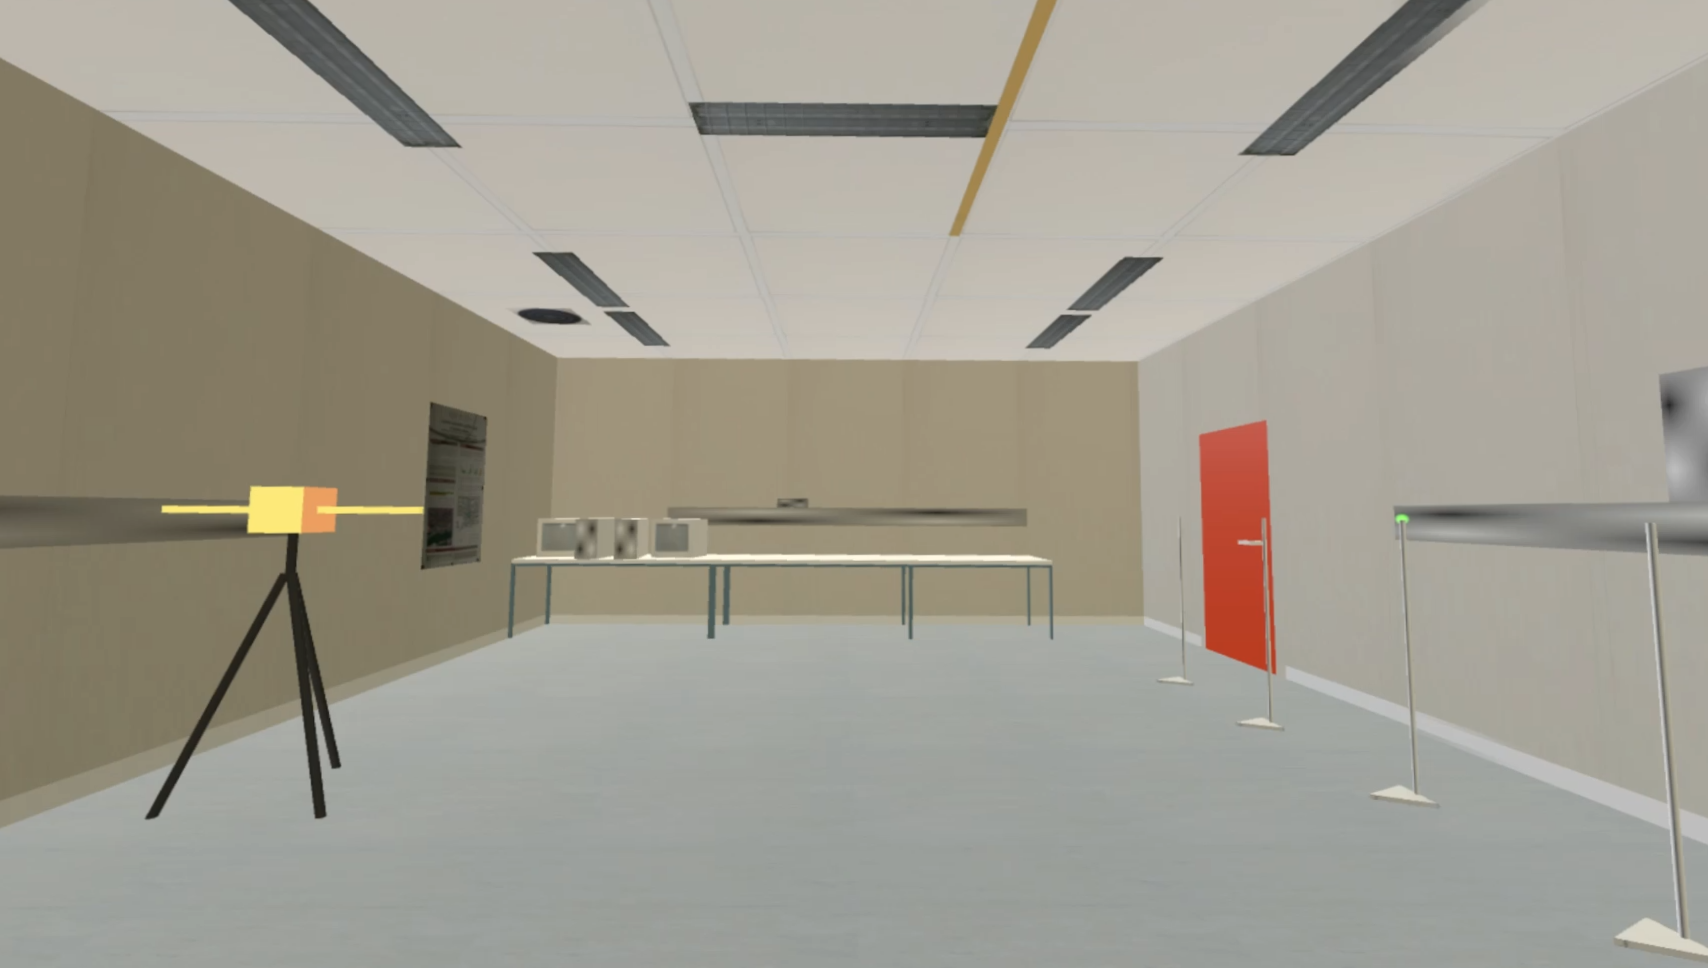
\includegraphics[width=12cm]{Images/SzenenBeispiel.png}
    \caption{Example virtual reality scene of the experiment in the light condition from the perspective of the subject.} 
    \label{SceneExampleLight}
\end{figure}
In the dark condition only the pointer and the target light were visible (see figure \ref{SceneExampleDark}). In the light condition the whole room, the pointer including its stand, the target light, and all five target-stands were visible at all times (see figure \ref{SceneExampleLight}). 
\begin{figure}
    \centering
    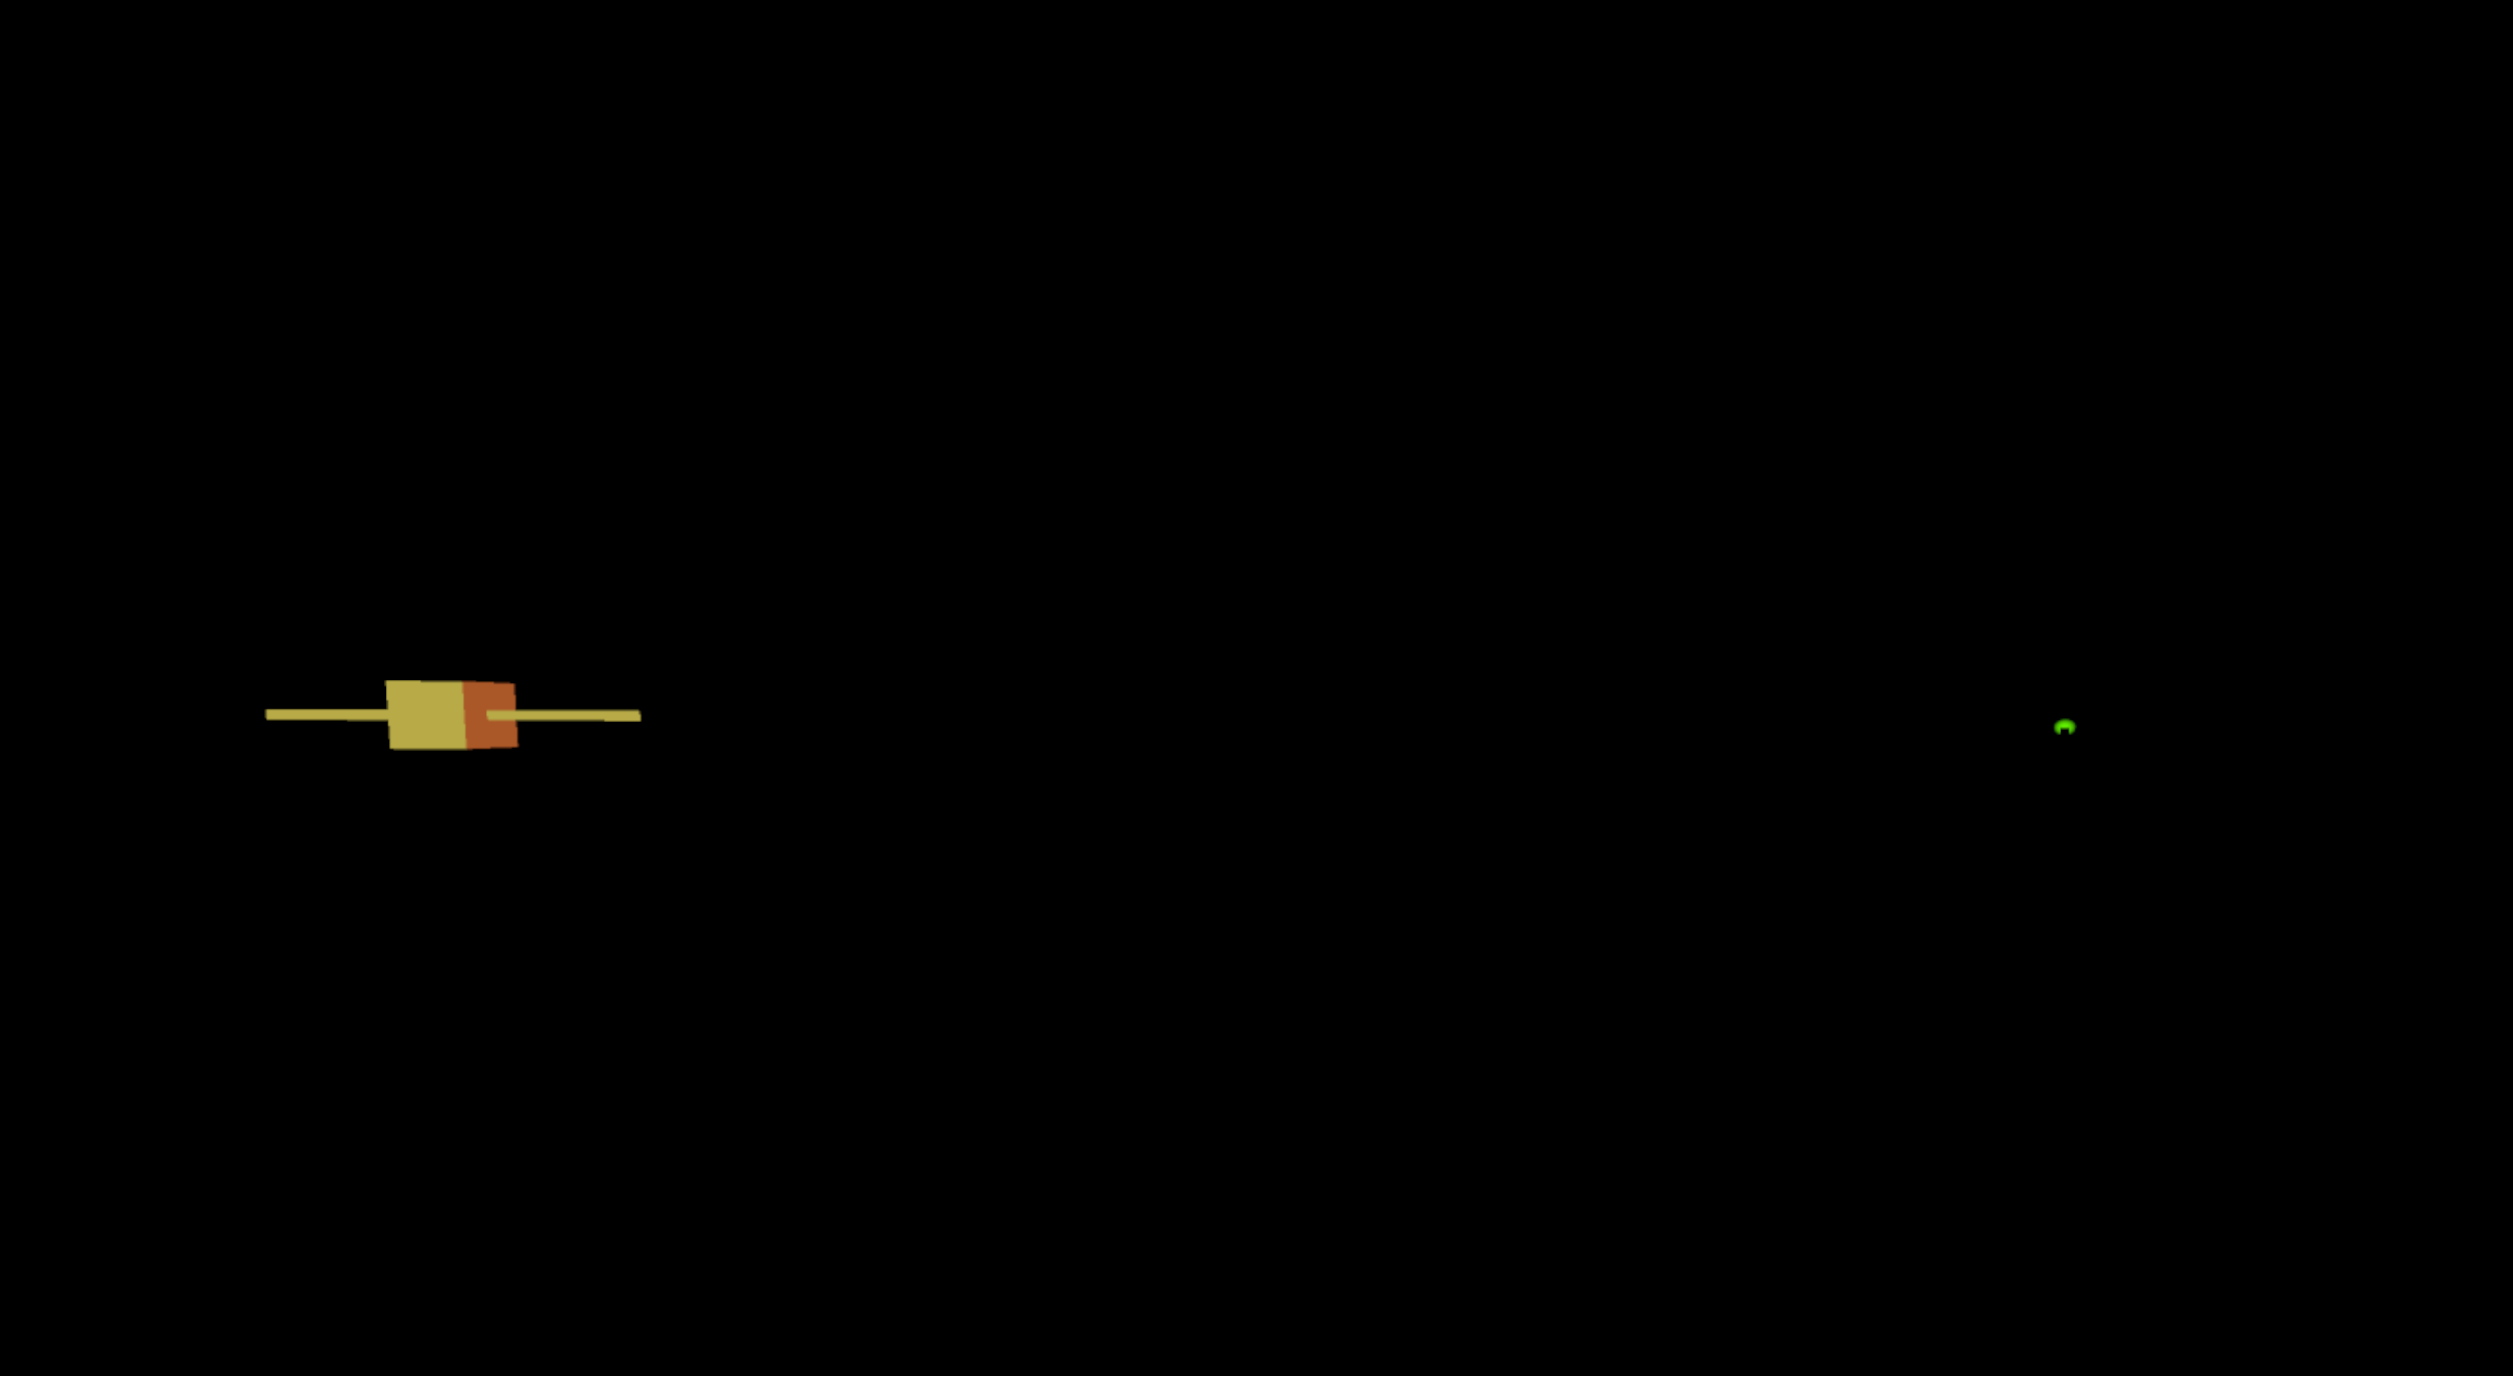
\includegraphics[width=12cm]{Images/SzeneDunkelBeispiel.png}
    \caption{Example virtual reality scene of the experiment in the dark condition, from the perspective of the subject. Note that only the pointer and the luminous target are visible.} 
    \label{SceneExampleDark}
\end{figure}

\begin{figure}
    \centering
    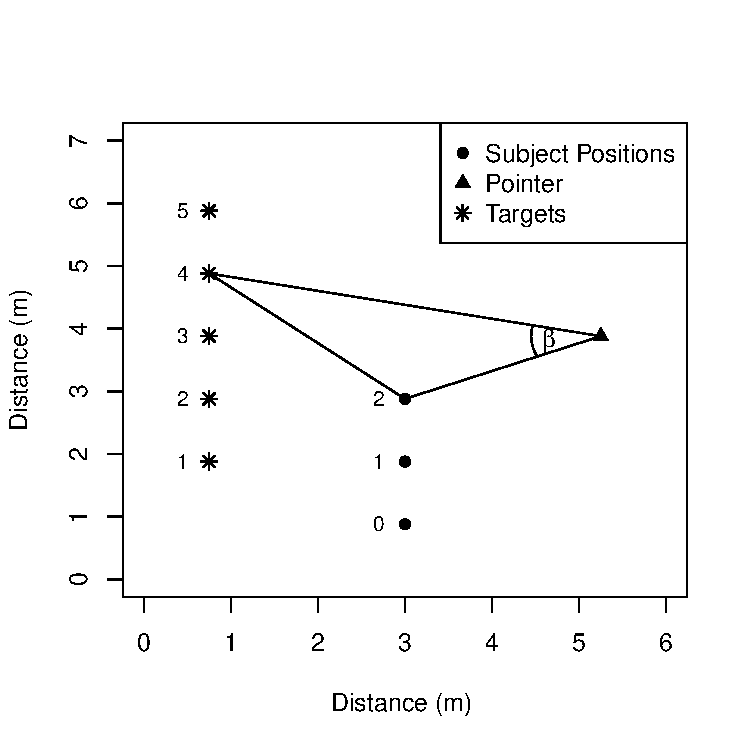
\includegraphics[width=8cm]{Images/schematicAufbau.pdf}
    \caption{Schematic image of the stimuli arrangement of the pointer right symmetry condition. Marked are the five targets, the pointer position, and the three different subject positions with $(0,0)$ marking the left rear corner of the room. Also indicated is the angle $\beta$ for one trial (subject position 2, target 4), which varied each trial depending on the target and the subject position.} 
    \label{SchematicAufbau}
\end{figure}

\section{Experimental procedure and design}
The subjects were tested in a single session of about 50 minutes ($\mu = 50.28, SD = 8.36$). Having given their informed consent, the subjects were given a controller for pointer-control, %dieser Satz ist zu lang
confirmation of set angle and pausing into their right hand and were instructed to orient the pointer towards the green light in their own time. They were able to adapt in the virtual room by some test trials (dark condition), in which they could explore the pointer control. Once they felt comfortable with handling the controller, the experiment started. In the beginning of the experiment the pointer was oriented towards the middle target stand, thus starting of in a 90\textdegree{} angle. Each trial the pointer orientation started off as it was set in the end of the preceding trial. The next trial started immediately after the subjects had confirmed the pointer's position in the preceding trial. The subjects were free to take as many breaks as they wanted. %nicht ideale überleitung zum letzten Satz


%design
The experiment was conducted as a within subject design. It consisted of 240 trials grouped into twelve blocks, in which lighting, pointer position, and subject position was varied.  Each block consisted of twenty trials, with each target-stand being targeted four times in a randomised order. The order of trials was kept the same for each block, condition and subject. The first six blocks were conducted in the dark, the later with lighting being present (dark and light condition). The experiment was symmetrically balanced with pointer and targets swapping sides after three blocks in both the dark and the light condition. In each of these blocks the subject was placed at a different position (see figure \ref{SchematicAufbau}). 

The manipulated variables were the angle $\beta$ (the angle varied between 0\textdegree{} and 77\textdegree{}) depending on the subject position and the target the subject was aiming at (see figure \ref{SchematicAufbau}), the pointer position (left or right), and the lighting (dark or light). In each frame the head rotation (x,y,z), the time stamp, and the pointer orientation angle were saved. 
%muss noch irgendwie rein:

Each of the subjects started with a different block. The first subject started at position 0 with the pointer to their left side, the second subject started at position 2 (descending subject position each block) with the pointer to their left side, the third subject at position 0 (ascending subject position each block) with the pointer to their right side, and the fourth subject started at position 2 with the pointer to their right side. All participants started with the dark condition.


% movement speed of pointer
\cleardoublepage
%############### RESULTS #########################

\chapter{Results}
\label{Results}
During the experiment, for each trial the reaction time and the pointer orientation were saved, when the subjects had confirmed the pointer's orientation. With the pointer's orientation the angle deviation from $\beta$ (see figure \ref{SchematicAufbau}) was calculated. The deviation was positive, when there was an overshoot of poin\-ting, and negative, when an undershoot was found.
All deviation values are given in degrees. 
All data was processed by using R. %muss das rein? 
Trials with a reaction time less than two seconds and no pointer movement were considered as accidental confirmation and excluded (one trial in total). 
The intrinsic curvature may be different for each subject. That is why the results are presented for each subject separately. The data of the subject who had already participated in the real life experiment is not included in the general results and only used to compare this experiment to the real life experiment. 


\section{Angle deviation}
For each target the deviation in each condition was measured four times, over which a mean was taken. In figure \ref{DeviationVP1} the mean deviation by $\beta$  of the first subject (VP1) is shown. In the dark condition with increasing $\beta$ there is a strong positive increase in the angle deviation, which slightly levels off at the highest angles. In the light condition, on the other hand, there is a small ditch into a negative deviation, which is then followed by a strong increase into a positive deviation. Note that some values of $\beta$ were only found for one or two subject positions, but there is still a continuous shape to be seen.


\begin{figure}
    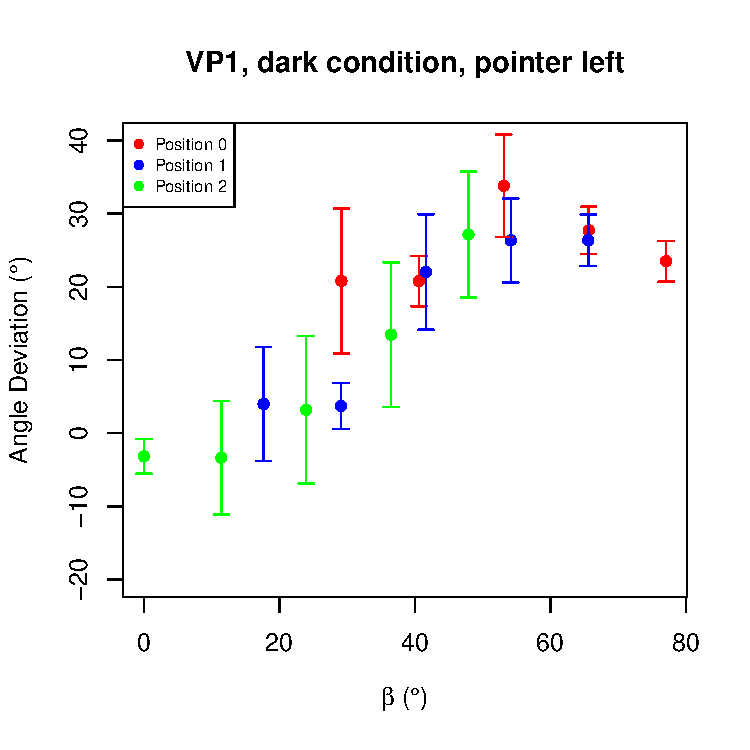
\includegraphics[width = 7cm]{Images/plots/AngleDevVP1DarkLeft.pdf}
    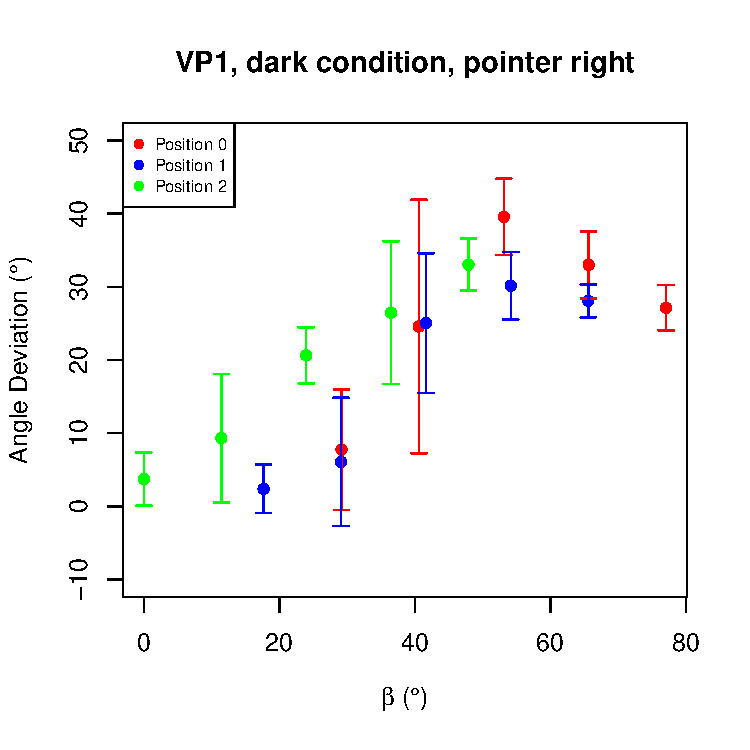
\includegraphics[width = 7cm]{Images/plots/AngleDevVP1DarkRight.pdf}
    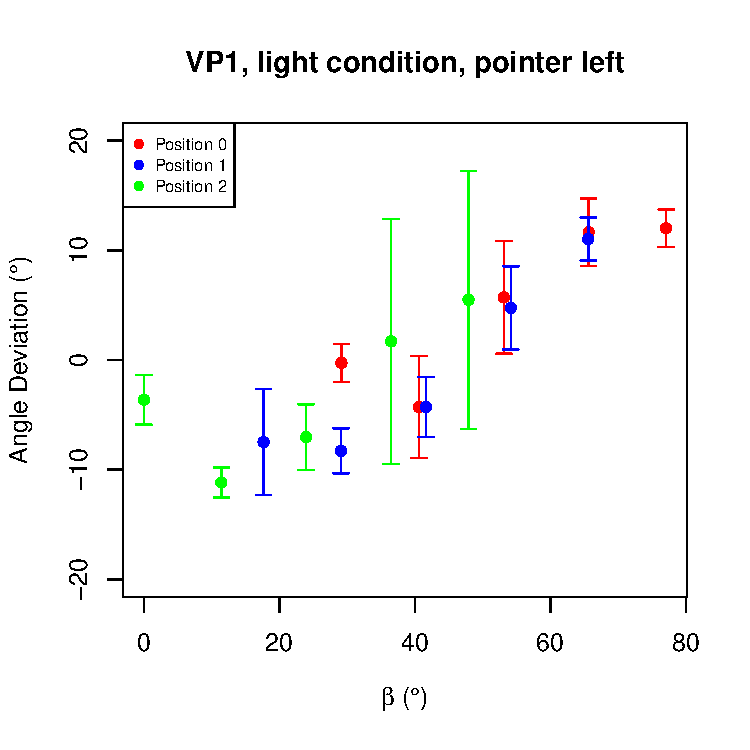
\includegraphics[width = 7cm]{Images/plots/AngleDevVP1LightLeft.pdf}
    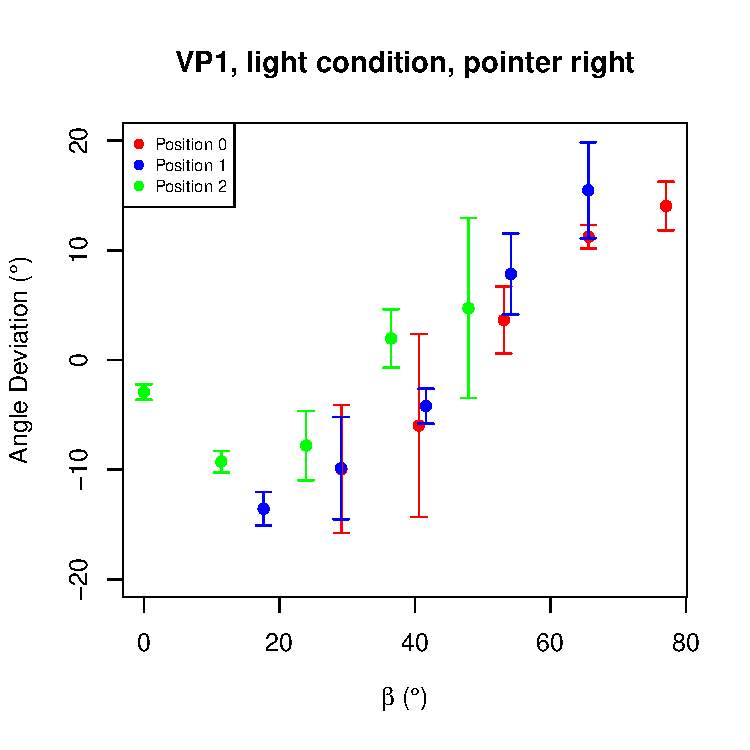
\includegraphics[width = 7cm]{Images/plots/AngleDevVP1LightRight.pdf}
    \caption{The mean angle deviation of the first subject (VP1) per pointer position and light condition (pointer left/right, lighting dark/light) for each subject position by $\beta$. Error bars indicate the standard deviation. Be aware of the partly different scale on the y-axis.} 
    \label{DeviationVP1}
\end{figure}
\begin{figure}
    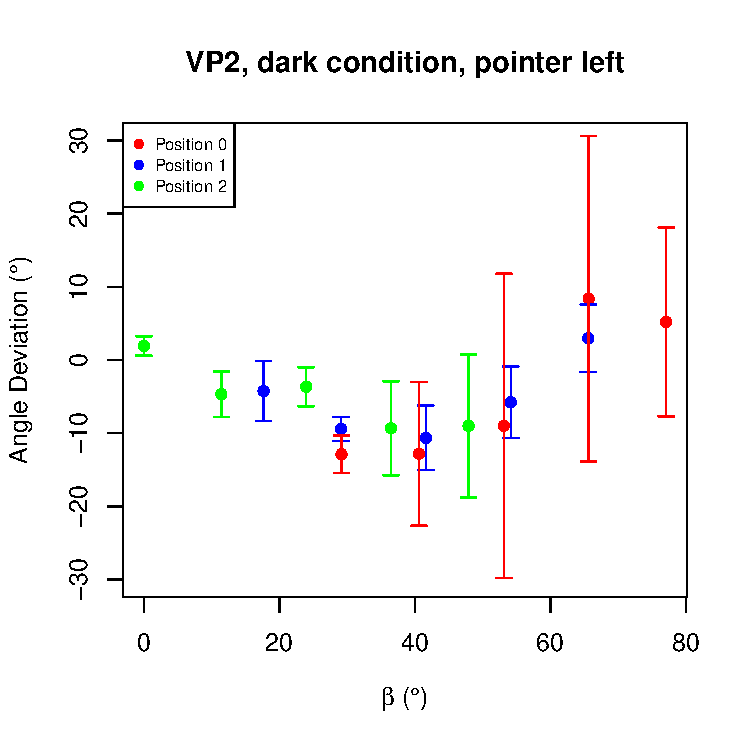
\includegraphics[width = 7cm]{Images/plots/AngleDevVP2DarkLeft.pdf}
    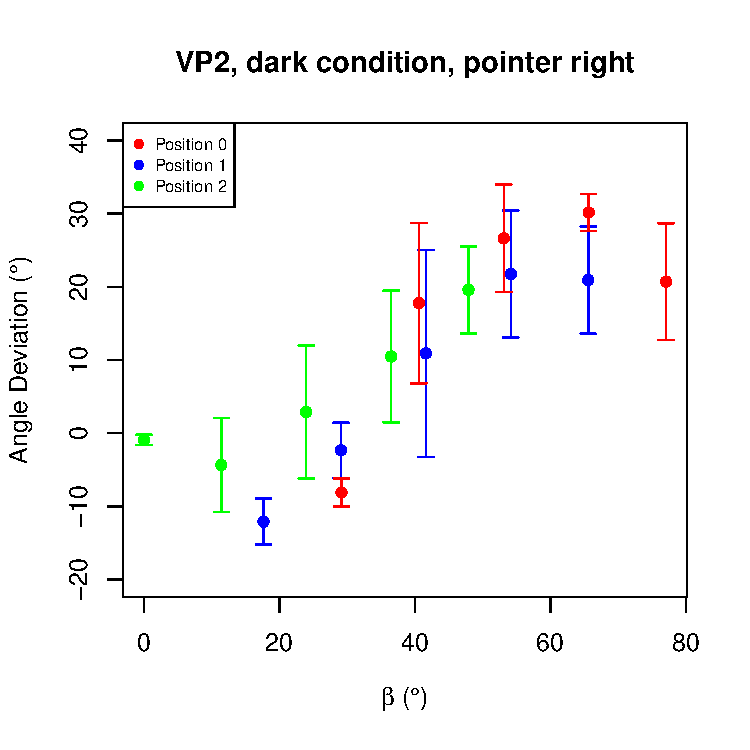
\includegraphics[width = 7cm]{Images/plots/AngleDevVP2DarkRight.pdf}
    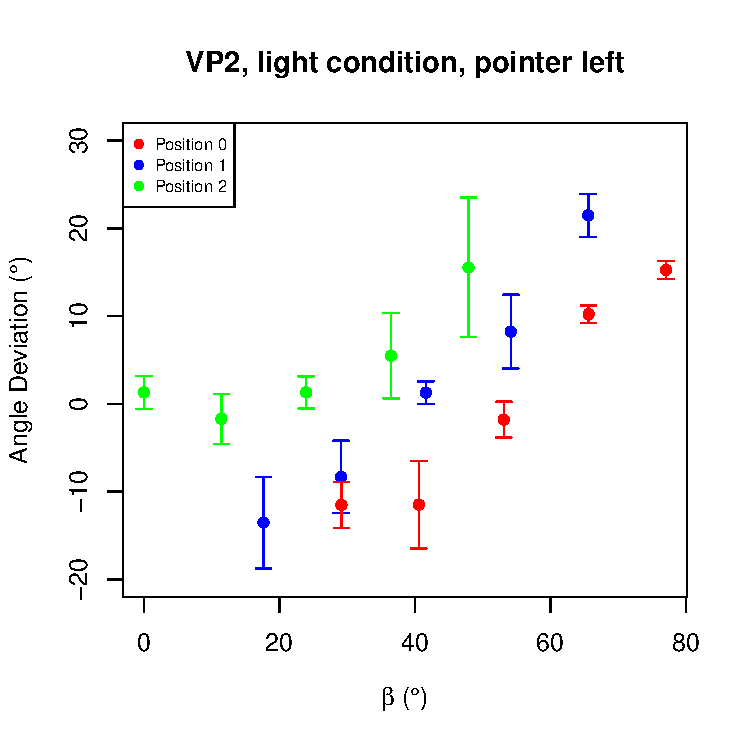
\includegraphics[width = 7cm]{Images/plots/AngleDevVP2LightLeft.pdf}
    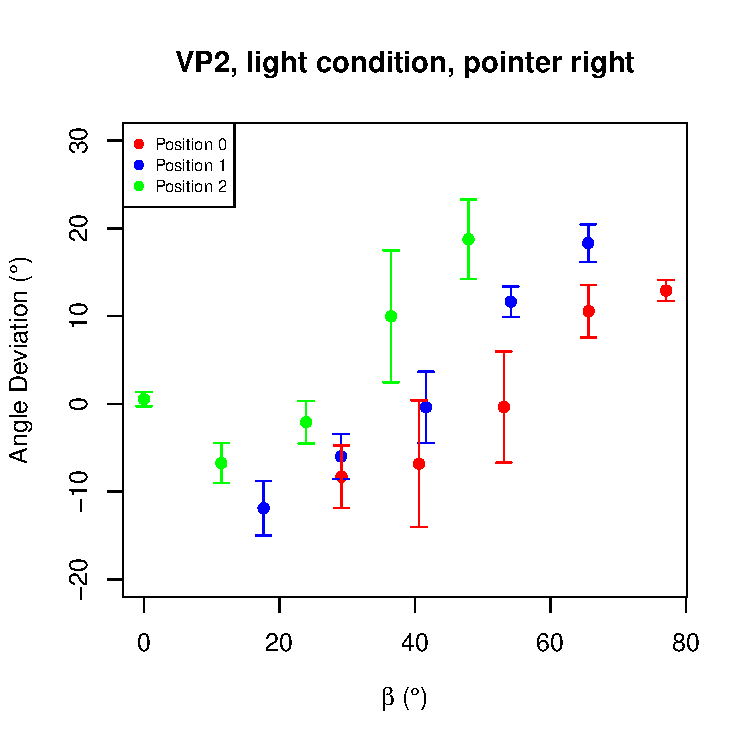
\includegraphics[width = 7cm]{Images/plots/AngleDevVP2LightRight.pdf}
    \caption{The mean angle deviation of the second subject (VP2) per pointer position and light condition (pointer left/right, lighting dark/light) for each subject position by $\beta$. Error bars indicate the standard deviation. Be aware of the partly different scale on the y-axis.} 
    \label{DeviationVP2}
    
\end{figure}
\begin{figure}
    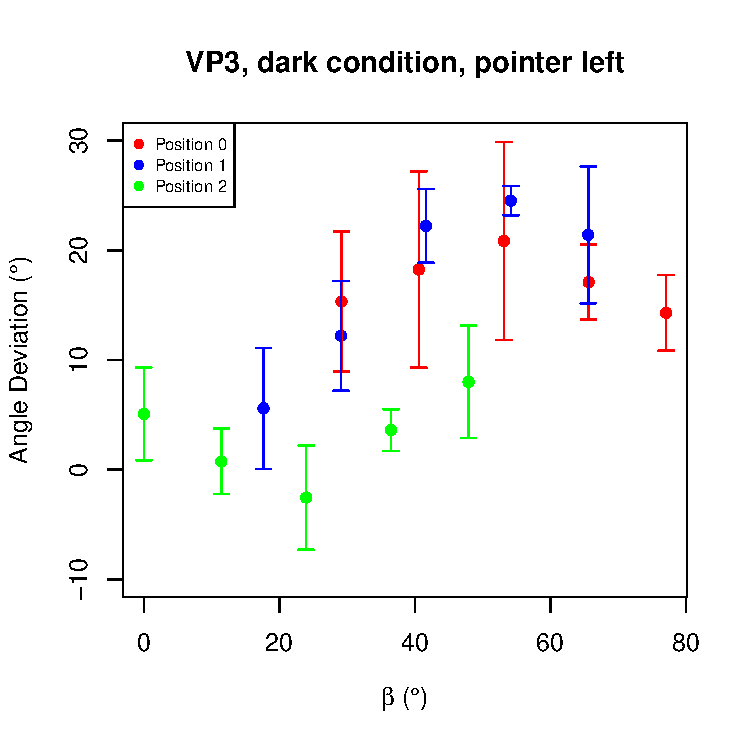
\includegraphics[width = 7cm]{Images/plots/AngleDevVP3DarkLeft.pdf}
    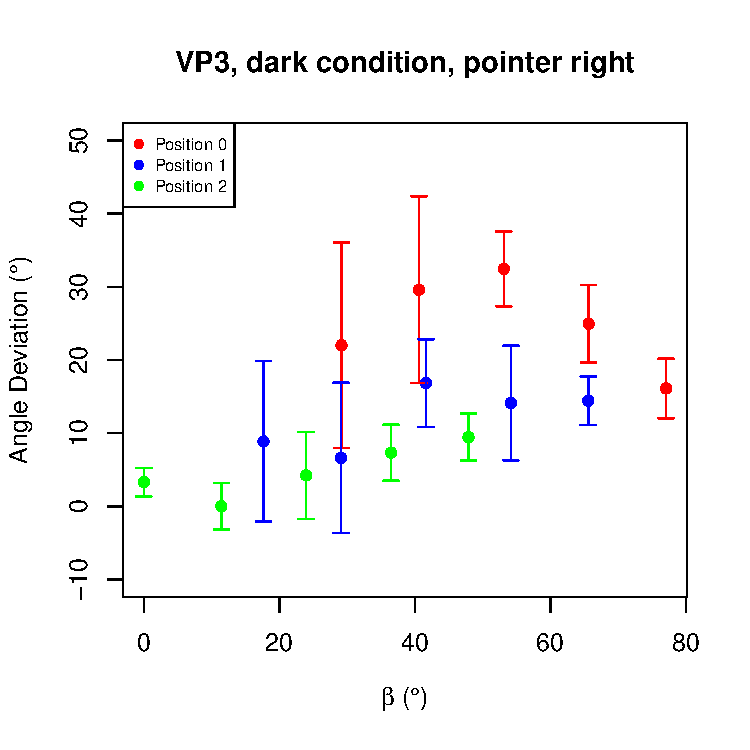
\includegraphics[width = 7cm]{Images/plots/AngleDevVP3DarkRight.pdf}
    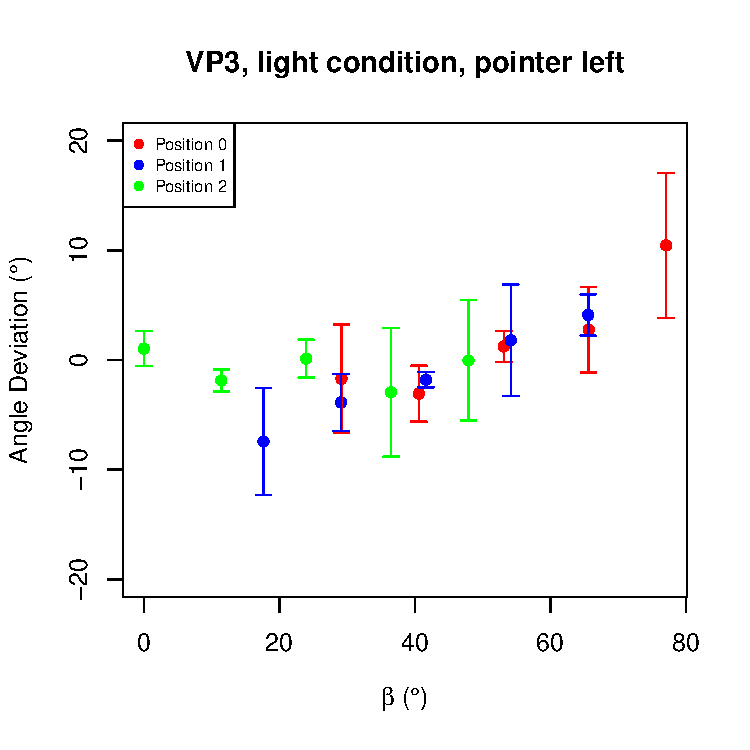
\includegraphics[width = 7cm]{Images/plots/AngleDevVP3LightLeft.pdf}
    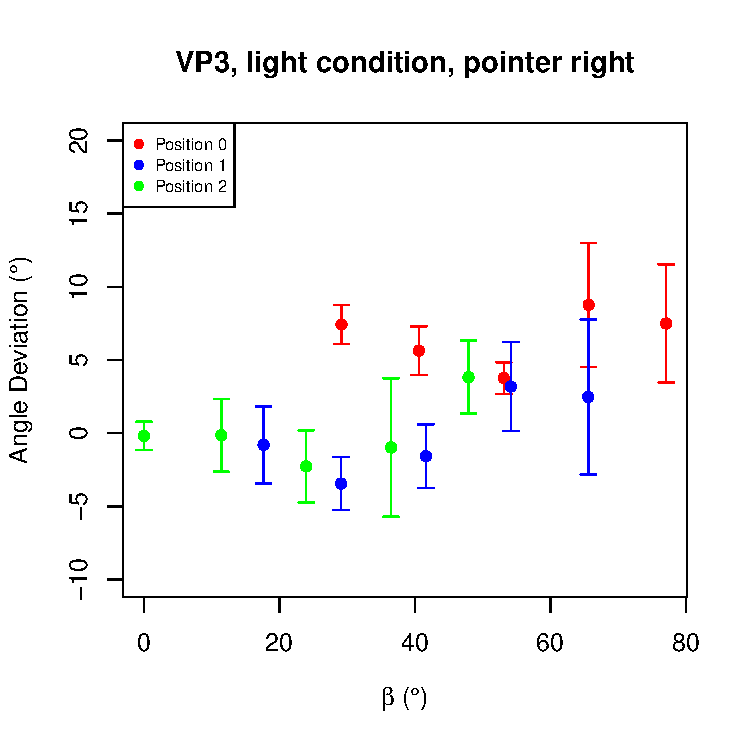
\includegraphics[width = 7cm]{Images/plots/AngleDevVP3LightRight.pdf}
    \caption{The mean angle deviation of the third subject (VP3) per pointer position and light condition (pointer left/right, lighting dark/light) for each subject position by $\beta$. Error bars indicate the standard deviation. Be aware of the partly different scale on the y-axis.} 
    \label{DeviationVP3}
\end{figure}
\begin{figure}
    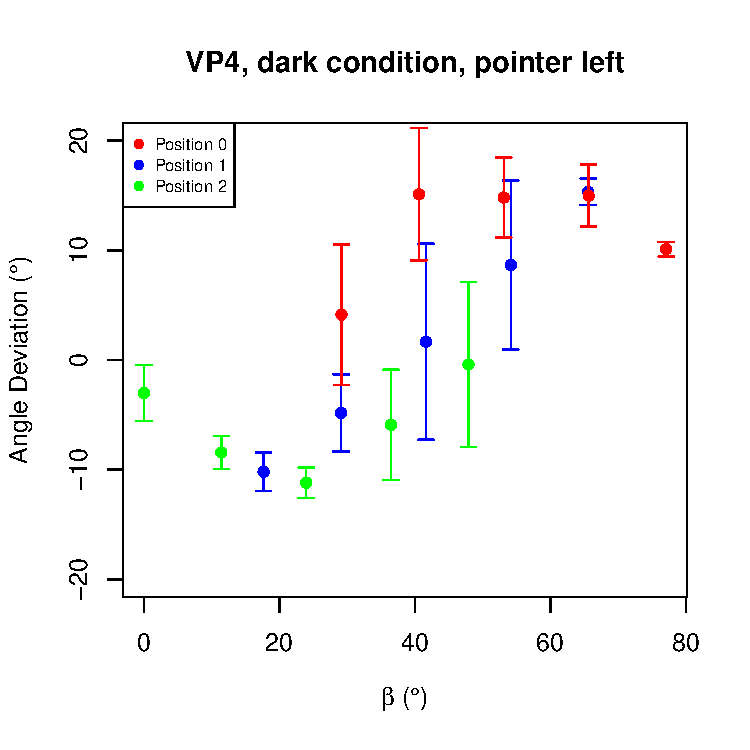
\includegraphics[width = 7cm]{Images/plots/AngleDevVP4DarkLeft.pdf}
    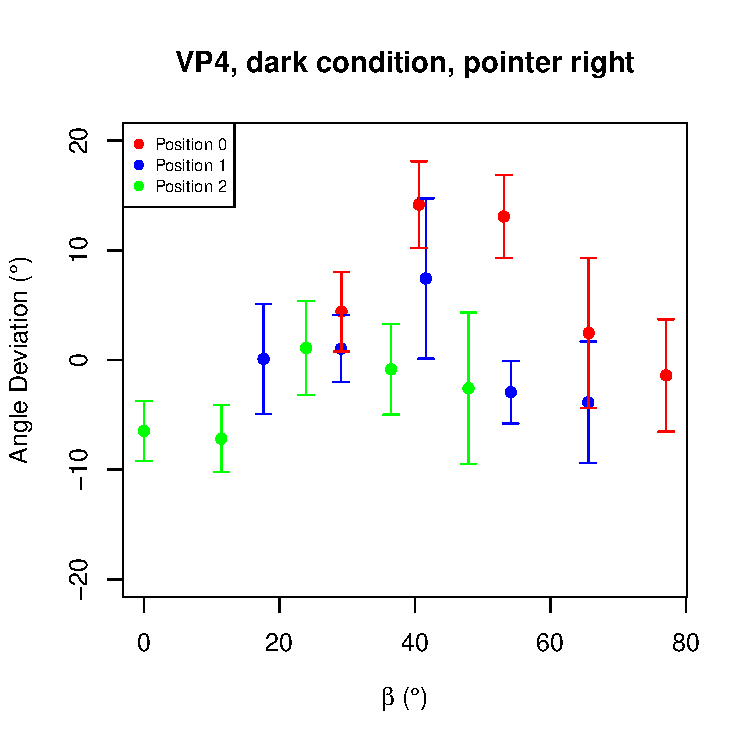
\includegraphics[width = 7cm]{Images/plots/AngleDevVP4DarkRight.pdf}
    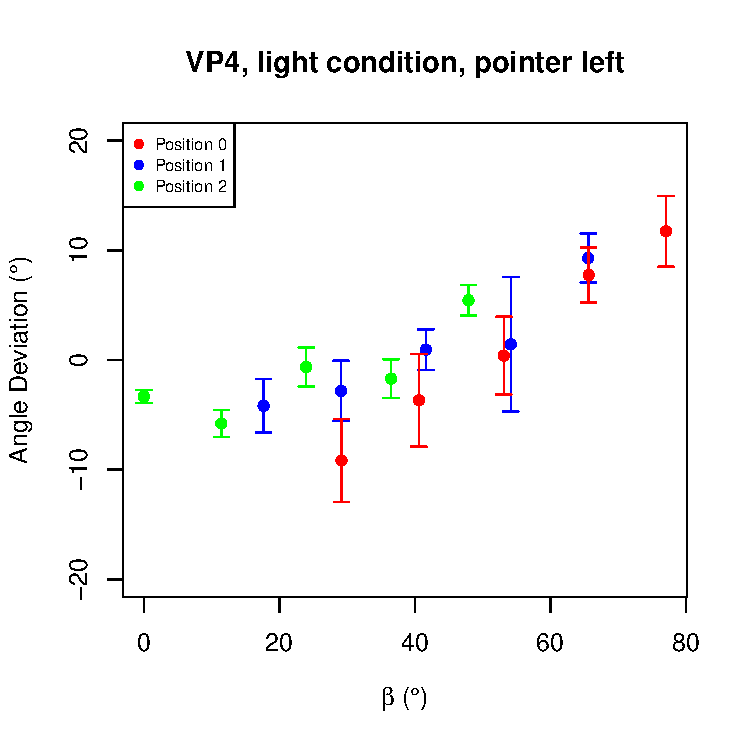
\includegraphics[width = 7cm]{Images/plots/AngleDevVP4LightLeft.pdf}
    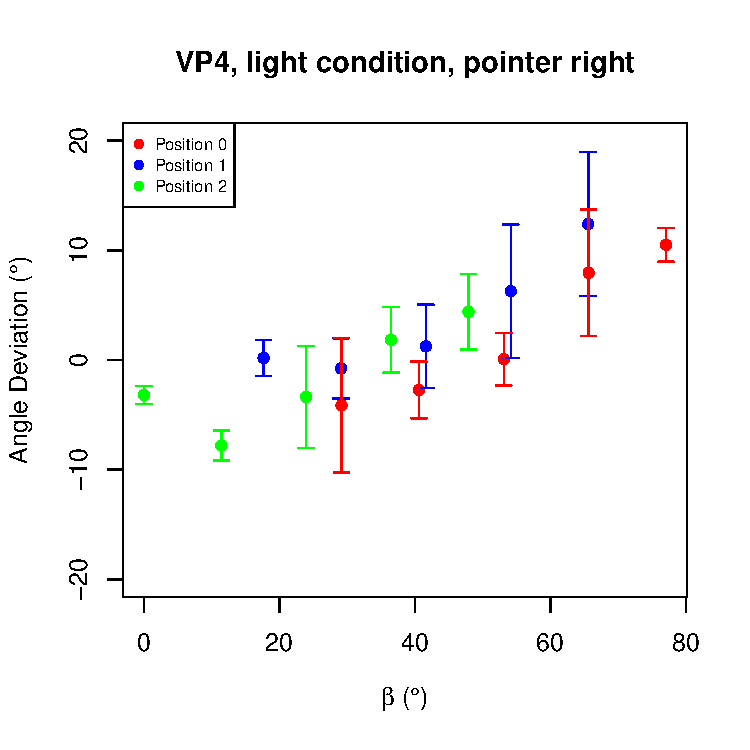
\includegraphics[width = 7cm]{Images/plots/AngleDevVP4LightRight.pdf}
    \caption{The mean angle deviation of the fourth subject (VP4) per pointer position and light condition (pointer left/right, lighting dark/light) for each subject position by $\beta$. Error bars indicate the standard deviation.} 
    \label{DeviationVP4}
\end{figure}

In figure \ref{DeviationVP2} the same is depicted for the second subject (VP2). Note that in the light condition for both symmetries the means can be distinguished with regard to the different subject positions (marked in red, green, and blue). A similar distinction of at least two subject positions can be seen in figure \ref{DeviationVP3}, showing the deviation of the third subject (VP3) in the dark condition. Also interesting is that VP3 had mainly very small deviations in the light condition. The same can be observed for the fourth subject (VP4) as seen in figure \ref{DeviationVP4}. The development of the deviation by $\beta$ for VP4 in the light condition is almost a straight, as the deviation in total is very small for most angles. 
Overall, all four subjects show a similar shape with negative deviations with a smaller $\beta$ and positive deviations as $\beta$ increases.

%beta
Deviations per conditions were compared using analyses of variance (ANOVAs) over the factors lighting, pointer position (symmetry), $\beta$, and subject position with a significance level of $p < .05$. They confirmed the observations of the graphs. For each subject the angle $\beta$ was very sig\-ni\-fi\-cant (VP1:$F(1,36) = 156.99, p < .001$, VP2:$F(1,36) = 95.87, p < .001$, VP3:$F(1,36) = 84.07), p < .001$, VP4:$F(1,36)= 95.09, p < .001$). This has been expected, having looked at the graphs, as the deviation indeed changes drastically depending on $\beta$.

%lighting
A main effect for the lighting could only be shown for VP1 and VP3, but in both cases it was very significant ($F(1,36) = 193.11, p < .001$ and $F(1,36) = 196.05, p < .001$ respectively). This is seen in figure \ref{DeviationVP1} and \ref{DeviationVP3} with a higher positive deviation for the dark condition than for the light condition.

%pointerPosition
The pointer position was very significant for VP2 ($F(1,36) = 33.68, p < .001$) and significant for VP3 $(F(1,36) = 4.95, p = .032$). That means these subjects did not show a symmetric deviation, the curvature depended on the side the pointer and the targets were placed. Figure \ref{VP2Symmetry} gives a deeper insight into the effect of the pointer position. %widerspricht meiner Kopfbewegungsidee. 
In this figure the difference of deviation (left pointer condition minus right pointer condition) by $\beta$ is depicted. It shows that for large values of $\beta$ the symmetry is not given. VP3 shows a similar but smaller effect. % should I also show the graphik for this VP

\begin{figure}
    \centering
    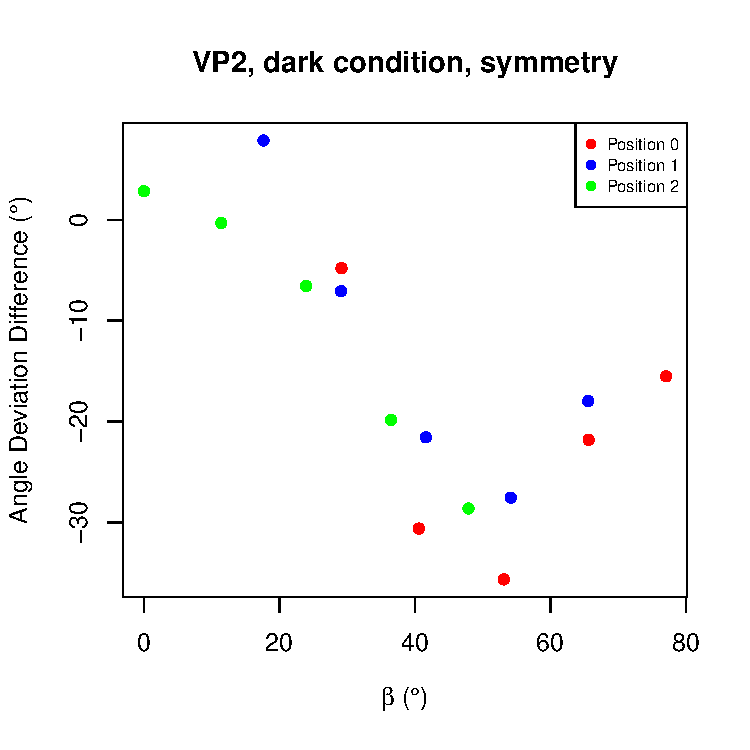
\includegraphics[width=7cm]{Images/plots/VP2Symmetry.pdf}
    \caption{The angle deviation difference (left pointer condition minus right pointer condition) for VP2 per subject position for the dark condition by $\beta$. If perfect symmetry was given, the values would be 0.}
    \label{VP2Symmetry}
\end{figure}

%subjectPosition
The position of the subject, i.e. the distance of the subject to the pointer and the targets, was very significant for VP2 and VP3 ($F(1,36) = 18.13, p < .001$ and $F(1,36) = 18.80, p < .001$ respectively), significant for VP1 ($F(1,36) = 3.49, p = .041$), and showed a tendency for VP4. For VP3 and VP4 this is clearly seen in the dark condition (figure \ref{DeviationVP3} and \ref{DeviationVP4}), for VP2 this effect can be seen in the light condition (figure \ref{DeviationVP2}) as in these graphs the different positions show different deviations for the same value of $\beta$.

This main effect of subject position cannot be set equal to the distance to the stimuli. The subject position only partly reflects the distance of the subject to the stimuli, as the distance not only depends on the subject, but also the target which is aimed at. Another representation of the deviation is in form of geodesics. It can be seen in figure \ref{VP1Curves}. The geodesics in these graphs have been approximated for each mean. The deviation was taken as the tangent for the circle arc. 
The scale of the different subject positions has been manipulated to enable the comparison of the different curves of different subject positions. Also the colour indicates the distance of the targets to the subject.  For example, target 1 in the graph of subject position 1 and target 2 in the graph of subject position 2 do have the same distance to the subject, and can hence be compared to check for the influence of the subject position. Figure \ref{VP1Curves} shows that overall the curvature is most elliptic for targets furthest away from the subject and becomes hyperbolic for targets closer to the subject. For example the red geodesic is slightly hyperbolic for all three subject positions. That means that for VP1 in the light right pointer condition a clear tendency of the influence of the subject's distance to the stimuli, i.e. not only to the pointer but also to the targets, can be seen.  

\begin{figure}
    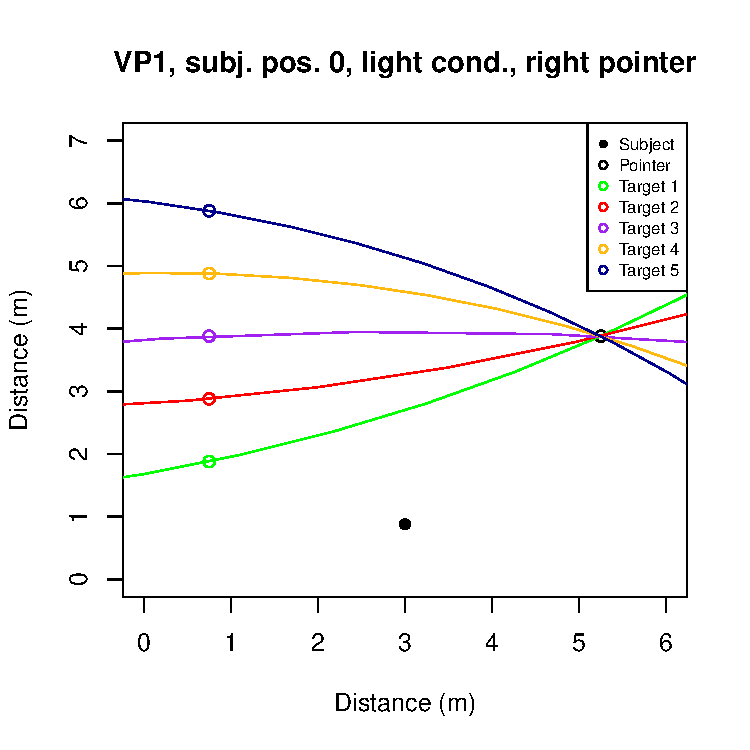
\includegraphics[clip, trim = 0.1cm 0.5cm 0.95cm 0.6cm, width=4.85cm]{Images/plots/VP1lightrightPos0Curves.pdf}
    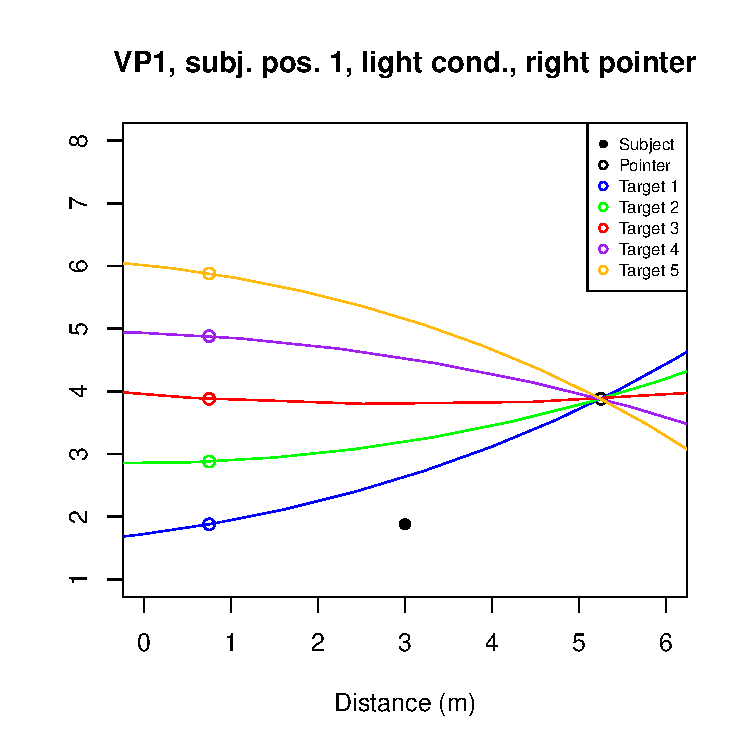
\includegraphics[clip, trim = 1.15cm 0.5cm 0.95cm 0.6cm, width=4.4cm]{Images/plots/VP1lightrightPos1Curves.pdf}
    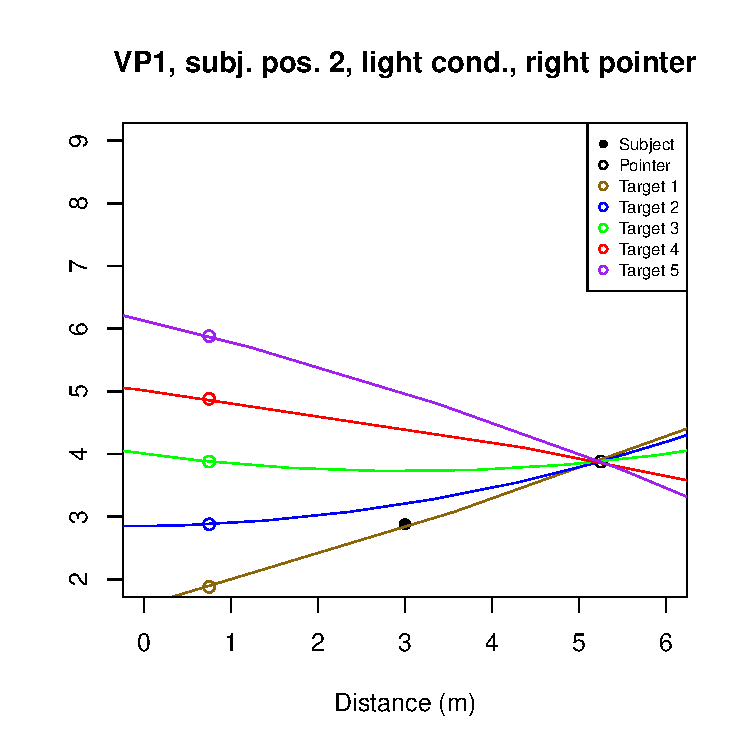
\includegraphics[clip, trim = 1.15cm 0.5cm 0.95cm 0.6cm, width=4.4cm]{Images/plots/VP1lightrightPos2Curves.pdf}
    \caption{The curvature of the intrinsic visual space approximated by geodesics for each target position for VP1 in the light, right pointer condition. The scale has been changed for each subject position to allow comparison of the curvature per distance of the subject to the targets. The colours encode for the distance of the targets to the subject. (0,0) marks the left rear corner of the room.}
    \label{VP1Curves}
\end{figure}

Additionally to these main effects, some interactions have been found. In the following only interactions between two factors will be discussed, even if some significant triple interactions have been found. Generally, interactions strongly depended on the subject, i.e. were only found significant for one or two subjects. The expected interaction between lighting and pointer position was only found to be significant for VP2 ($F(1,36) = 29.09, p < .001$) and a tendency was found for VP1. Note that VP2 was also the only subject who showed a very significant effect of pointer position. Interesting %worwahl (Augen verdrehen)
is a very significant interaction of lighting and subject position for VP2, VP3, and VP4 ($F(1,36) = 6.78, p = .032, F(1,36) = 15.21, p<.001$ and $F(1,36) =17.87, p < .001$ respectively). Also unexpected is a very significant interaction between the pointer position and the subject position for VP3 ($F(1,36) = 8.58, p<.001$) and a tendency for this interaction for VP1.
And finally for VP2 a very significant interaction ($F(1,36) = 6.83,p = .0031$), for VP3 a significant interaction ($F(1,36) = 5.12, p = .011$) and a tendency for VP1 between $\beta$ and the subject position was found. As $\beta$ directly depends on the subject position, this is not surprising. 
%sollte ich F-Werte bei Tendenzen angeben?

%Interaction pointer position and $\beta$. TODO wo erwähne ich die denn in der Diskussion?

\begin{figure}
    \centering
    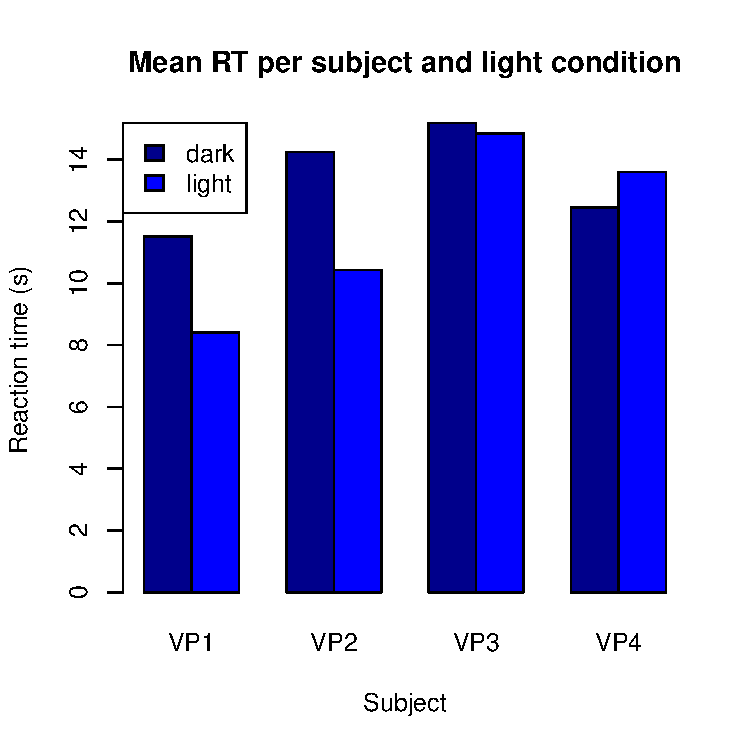
\includegraphics[width=7cm]{Images/plots/ReactionTimes.pdf}
    \caption{The mean reaction times per subject and light condition in seconds.}
    \label{ReactionTime}
\end{figure}

\section{Reaction time}
The reaction time per trial does not have a great informative value, as the time to rotate the pointer is included in the reaction time. For example, once per block the subjects pointed at target 1 right after pointing at target 5. This takes much longer than to rotate the pointer to target 1 from target 2. This results in a great variation of the reaction time values. While the mean over all subjects in seconds is $12.58$, the standard deviation is almost as high ($SD = 10.24$). Even so, the reaction time can be compared as means per condition.

The difference of the reaction time in the dark and the light condition per subject is shown in figure \ref{ReactionTime}. It shows that most subjects were faster in the light condition. This was confirmed by a two-sided paired t-test. Over all subjects the reaction time in the light condition was significantly shorter than in the dark condition ($t(478) = -2.60, p = .0097$). It is interesting to note that VP3 and VP4, who show a similar reaction time in both lighting conditions, are also those who showed only small deviations in the light condition (see figures \ref{DeviationVP3} and \ref{DeviationVP4}). 


\section{Comparison to real life experiment}
To compare this experiment to the real life experiment and hence to examine the usefulness of virtual reality for our research question, the data of the subject which participated in both experiments was compared. In figure \ref{DeviationBOTHVP5} the mean deviation by $\beta$ of this fifth subject (VP5) is shown for both the real life experiment (RL) and the virtual reality experiment (VR). The values of the two experiments can be distinguished by colour and symbol shape. In the light condition the deviation is surprisingly similar. For the left and the right pointer condition especially the deviations on subject position 2 are almost identical, the means of which can be distinguished from the other subject positions. In the dark condition in the pointer right condition a similar overlap can be seen, while on the other hand in the pointer left conditions great discrepancies are visible. In this condition in VR the deviation has relative smaller values for $\beta$ greater than 20\textdegree{} than in RL. Particularly interesting is that, while the deviations of subject position 0 remain fairly similar, the deviations of subject position 1 and 2 are very different. Overall, VP5 provided similar deviations in both experiments.
% Discussion: leading to the conclusion, that VR is indeed a possible measurement for the intrinsic geometry of the visual space. %Discussion?


\begin{figure}
    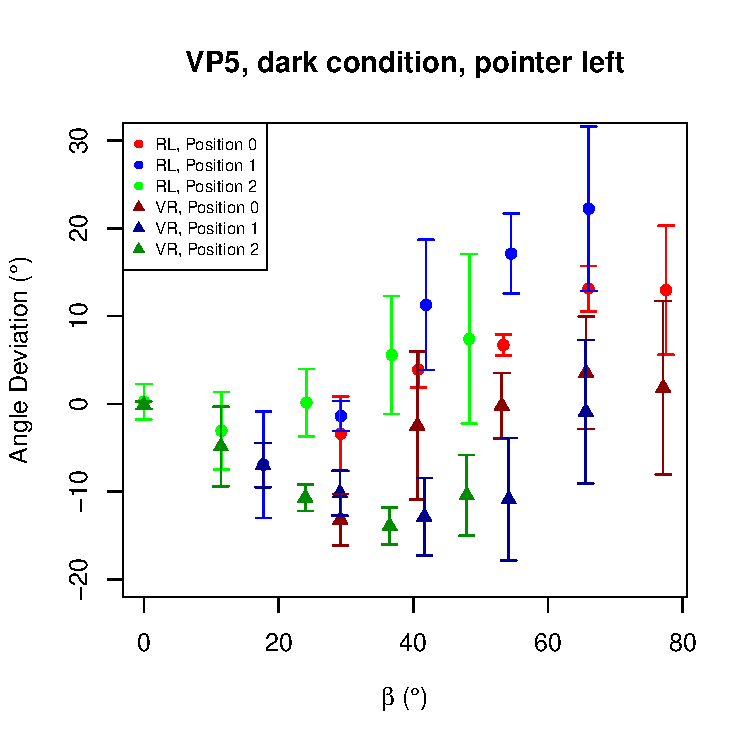
\includegraphics[width = 7cm]{Images/plots/AngleDevVP5BOTHDarkLeft.pdf}
    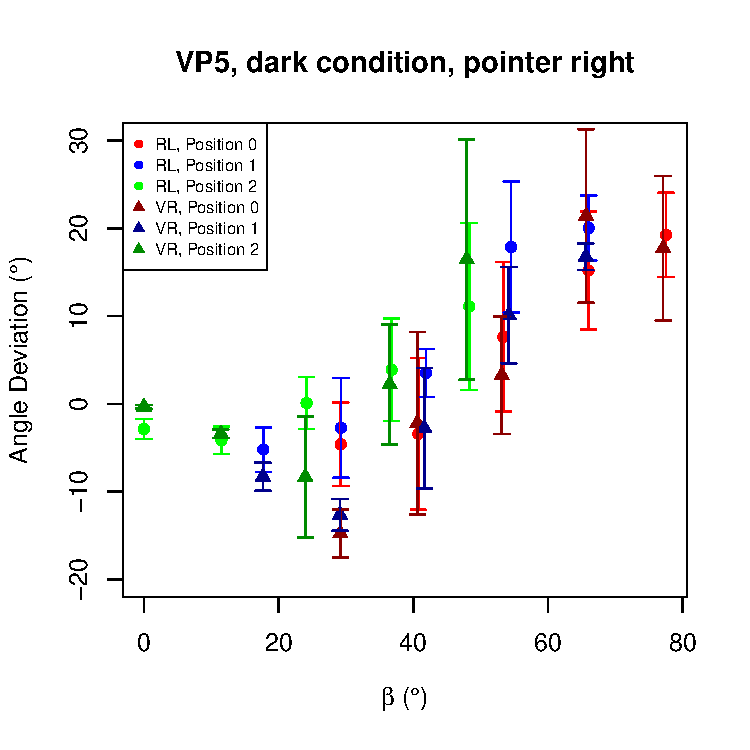
\includegraphics[width = 7cm]{Images/plots/AngleDevVP5BOTHDarkRight.pdf}
    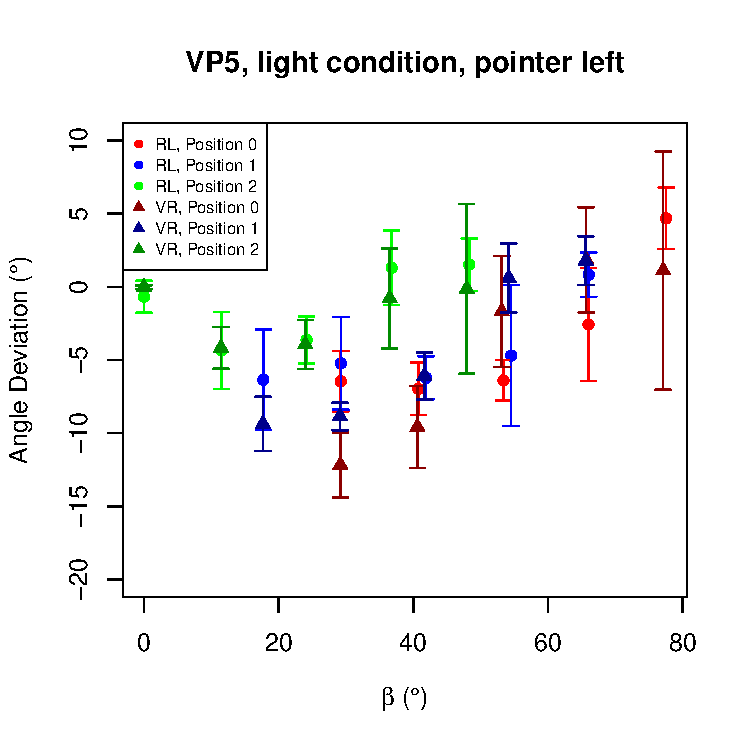
\includegraphics[width = 7cm]{Images/plots/AngleDevVP5BOTHLightLeft.pdf}
    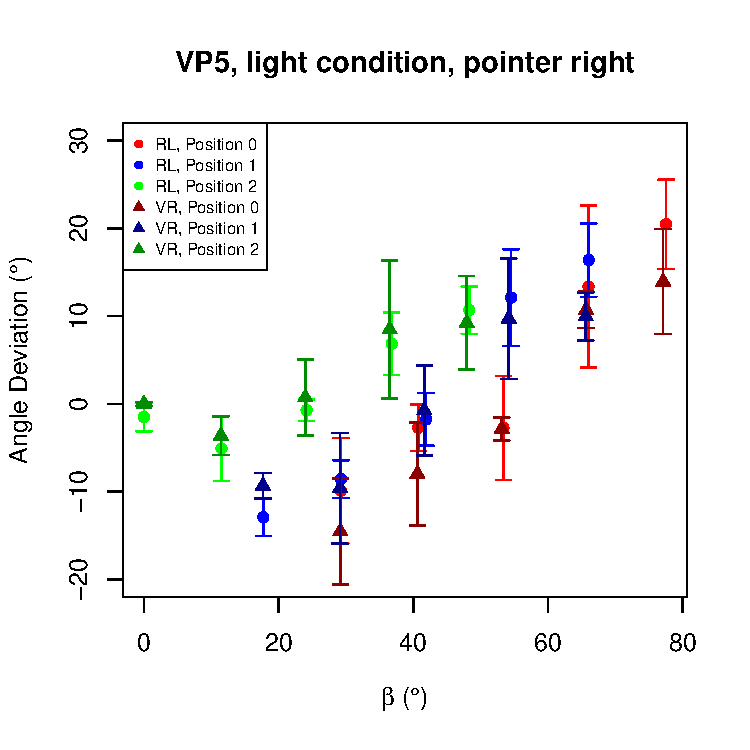
\includegraphics[width = 7cm]{Images/plots/AngleDevVP5BOTHLightRight.pdf}
    \caption{The mean angle deviation of the fifth subject (VP5) per pointer position and light condition (pointer left/right, lighting dark/light) for each subject position by $\beta$ for both the real life experiment (RL) and the virtual reality experiment (VR). Error bars indicate the standard deviation. Be aware of the partly different scale on the y-axis.} 
    \label{DeviationBOTHVP5}
\end{figure}


%For this purpose one of the subjects participated in the real life experiment, will also take part in this experiment. Obviously this subject cannot be counted as naive subjects, but as the curvature of the visual space varies per person, hence comparison of data of different subjects is difficult, this may be the best possibility to compare the impact of doing the task in virtual reality in contrast of doing it in real life. 

% HeadMovement?






% values of beta instead of angles of beta.

%always say point instead of aim

%hier falsche wortwahl mit positive and negative curvature, instead elliptic and hyperbolic

%nai\"{}ve
\cleardoublepage
%%%%%%%%%%%%%%%%%%%%%%%%%%%%%%%%%%%%%%%%%%%%%%%%%%%%%%%
%%%%%%%%%%%%%%%%% DISCUSSION %%%%%%%%%%%%%%%%%%%%%%%%
%%%%%%%%%%%%%%%%%%%%%%%%%%%%%%%%%%%%%%%%%%%%%%%%%%%%%%%

\chapter{Discussion}
\label{Discussion}

This experiment investigated the intrinsic geometry of the visual space by exocentric pointing in a virtual reality. It examined if the geometry is of constant curvature as proposed by Luneburg \citeyear{Luneburg.1947}. The aim was to both show similar results as Koenderink et al. \citeyear{Koenderink.2000} and to test if geodesics are indeed the best way to describe the curvature. The study looked at different factors possibly influencing this geometry such as the lighting, the angle in which the pointer is standing relatively to the targets and the subject ($\beta$), and the side on which the pointer is standing. Additionally, it was tested if virtual reality is a possible measure for examining the intrinsic geometry of the visual space. 

We have shown in our experiment that there was a main effect of $\beta$ for all subjects, a main effect for lighting, pointer position, and subject position for some subjects. Additionally to these main effects, some interactions have been found. Only for VP2 the interaction between pointer position and lighting was significant. Furthermore, an interaction between lighting and subject position was found for most subjects, an interaction between pointer position and subject position, and an interaction between $\beta$ and subject position was found for some subjects. 
Over all subjects %Formulierung
the reaction time was significantly shorter for the light condition.
Finally, a comparison of the data of VP5 showed similar deviations for our VR experiment as for the RL experiment. 

Hereby our main hypothesis, that the intrinsic visual geometry is of no constant curvature, can be supported by our data. Luneburg's theory of a constant hyperbolic curvature \citeyear{Luneburg.1947} seems to become more unlikely. But while our deviation generally shows dependence on the subject position, figure \ref{VP1Curves} shows particularly well how our results oppose preceding research and our hypothesis that the curvature is elliptic in near space and hyperbolic in far space.
The curvature of the visual space, when plotted depending on the distance of the subject to the target, is hyperbolic in near space and elliptic in far space in our experiment, which is directly the opposite to the results of Koenderink et al. \citeyear{Koenderink.2000}. They showed the visual space to be elliptic in near space and hyperbolic in far space. 

This contradiction could partly be justified by the different experimental conditions. Only the light condition can be compared to their experiment. The experiment of Koenderink et al. \citeyear{Koenderink.2000} took place in the field, hence under natural conditions just as in our light condition. There were still some differences between these experiments. Firstly, the tested distance between subject and targets varied only from 2.23m to 5.47m in our experiment in comparison to a few to over 20m in the experiment of Koenderink et al. \citeyear{Koenderink.2000}. Secondly, in our experiment the sight was very limited by walls and furniture, which all provided monocular depth cues. The effect of these should not be underestimated since in our experiment the dark and light condition showed significantly different deviations for some subjects. Overall this is still not enough to explain the contradictory results. 
But looking at the greater picture %Formulierung
it could be shown that the geometry of the intrinsic visual space has a curvature and that it is not constant. The possible influence of factors other than distance will be discussed in the following. 

The main effect of $\beta$ for the deviation cannot be explained easily. As $\beta$ directly depends on the subject position and the target, it is not clear if this main effect is indeed due to the angle, i.e. the perspective the subject is having on the target and the pointer, or due to one of its dependent factors. 

The curve of the deviation by $\beta$ shows a relative decrease of the angle deviation value in the beginning, a strong rise and a slight decrease at the highest values of $\beta$ (see e.g. figure \ref{DeviationVP1}). It must be said that this shape is particularly defined by the deviation values at very low and very high values of $\beta$, which are only supported by few data.
%fewer data or less data. only small data samples?
Leaving out these two extreme values, for some subjects one could only speak of a linear shape of the deviation. Especially the deviation values at $\beta = 0$ should be handled with care. The value $\beta = 0$ means that the pointer, the target, and the subject were in one line; the subject was directly pointing at themself when pointing at the target. Hence, this was rather an aiming task, which is much easier than exocentric pointing. This could explain the deviation being closer to $0$ for all subjects and small error bars. This gives thus the possibly incorrect impression of a decrease at lower values of $\beta$. Therefore, one should rather speak of a tendency of these decreases at the extreme values of $\beta$ and should put the general linear increase into focus.

If, on the other hand, the slight decrease of the deviation at high values of $\beta$ is the beginning of a strong decline, then our results could still be compatible with those of Koenderink et al. \citeyear{Koenderink.2000}. One could imagine that the visual space is hyperbolic in very near space, elliptic in near space, but again hyperbolic in far space. The data collected in this experiment is not sufficient to tell anything about this assumption. Further research should again focus on the type of curvature depending on the angle or the distance between subject and stimuli.

In general, the experimental setting allowed only small data sets to be comparable as many factors were varied such as the target and thus only few trials were made under the exact same conditions. This was due to the limiting size of the lab room. Using virtual reality will resolve this limitation for future experiments. In similar experimental settings one should make sure that all angles are supported by data of at least two subject positions. This could be achieved by varying the distance between pointer and target as it has been done in the experiment of Koenderink et al. \citeyear{Koenderink.2000}.

% ditch is no professional expression for sure
Another factor we tested was the influence of monocular depth cues on the curvature. For this purpose we changed between the light and the dark condition. The lighting was very significant for VP1 and VP3. This means, for these subjects the cues given by the room did influence how they perceived depth. Both had relative larger values in the dark condition. For VP1 the small relative decrease of the deviation seen at the smaller values of $\beta$ disappears in the light condition (see figure \ref{DeviationVP1}). In this condition the deviation tends to be positive for all values of $\beta$. An explanation for this cannot be given easily. But as the only difference in the two conditions is the additional information provided by the room, the room structure must be the reason for these more positive deviations. Therefore, in our experiment in the dark condition the visual space is mainly elliptic for some subjects, while in the light condition it is hyperbolic at small values of $\beta$ and elliptic at high values of $\beta$.

For VP3, on the other hand, the deviation is generally smaller in the light condition than in the dark condition (see figure \ref{DeviationVP3}). Taking into account that VP3 is a subject who also had similar reaction times in the light and the dark condition (see figure \ref{ReactionTime}), one could assume that this subject in contrast to the others makes better use of the monocular cues for determining the ideal pointer's orientation. In theory, there were enough cues given (such as seeing that the middle target is directly opposite of the pointer) so that one could approximate the ideal orientation very well. I propose that VP3 indeed tried this, which took them more time, but resulted in a more accurate pointer orientation, i.e. smaller deviations. With the same argument one can explain the reaction time and the deviation of VP4.

Another difference between the dark and the light condition can be seen when looking at the symmetry. The side  the pointer was standing at influenced the deviation for some subjects. Looking at this factor of symmetry we got results opposing our hypothesis. We expected the deviation to be symmetrical in the dark and possibly less symmetrical in the light condition. Our data shows directly the opposite. The pointer position (left or right) was significant for VP2 and VP3. But in both cases it was the dark condition in which they showed less symmetry, as an interaction between lighting and pointer position is given at least for VP2.

These results question the general assumption that the geodesic alone is enough to describe the curvature of the intrinsic visual space, because symmetry must be given if one wants to describe the curvature using geodesics. One must add that this is the first experiment showing such an asymmetry. In all preceding experiments symmetry was found and hence assumed. Therefore it is particularly important to wonder about what kind of factors could have made this asymmetry possible in our experiment.

Figure \ref{VP2Symmetry} can lead to the assumption that the symmetry depends on $\beta$, thus that fewer symmetry is found for greater values of $\beta$. As already said, as $\beta$ depends on the target and the subject position, no further exploration of this assumption can be made. The symmetry may thus also depend on the subject position as the interaction between pointer position and subject position for VP3 would suggest, but it cannot be said confidently. 

One possible explanation for the greater symmetry in the light condition is that the room provided more depth cues, hence more cues for the position of the target. On the other hand, the data suggests that in the dark condition the subjects were not able to determine a constant position of the targets. It seems that in this experiment binocular vision as the only depth cue is not enough to determine the position of one luminous light. Luneburg gives support for this thought, stating that experiments with an isolated point in the dark showed that "binocular observation of a single point does not differ from monocular observation" \cite[p.~629]{Luneburg.1950}. This is a major criticism of our experiment. Especially in virtual reality, in which the field of view is limited, this could have a great impact. Subjects had to turn their heads away from the pointer in order to see the target. In no trial both the target and the pointer were fully visible in one field of view. Hence the subjects were very often looking at isolated points in the dark and Luneburg's critique can be applied. 

Extending the remark on the limited field of sight, the small distance between stimuli and subject leads to many head movements. This means that an interaction such as for example between lighting and subject position may in fact be an interaction between lighting and head movements, caused by limited sight. To investigate this, the tracked head movements could be examined and be tested for a correlation to the angle deviation. 

At last, we expected our VR experiment to have similar results to the RL experiment. Our expectations were met: both experiments showed very similar results for VP5 (see figure \ref{DeviationBOTHVP5}). Especially in the light condition the deviations are extraordinarily similar. Therefore, one can claim that it is possible to measure the intrinsic geometry of the visual space by using virtual reality. Only in one condition the deviations scarcely overlap. The reason for this could be the order in which the trials were presented. VP5 started with the pointer left condition while being placed at subject position 2, i.e. the closest one to the pointer. This is the subject position in which most head movements have to be made in order to see the target and could thus be called the subject position with the most difficult trials. At this point in the VR experiment the subject has no clear conception of the room the trials are placed in, as these were the first trials. This idea is supported by figure \ref{DeviationVP2} as VP2, starting with the same condition as VP5, also shows asymmetry comparing the dark pointer left condition with the dark pointer right condition. 

In contrary, in RL the light condition was done before the dark condition and therefore the subjects were able to get an impression of the position of the targets and the room dimensions.
This may have led to these strongly differing deviations in the pointer left dark condition, whereas in the other conditions VP5 showed very similar results in both experiments. Of course one subject is not enough to make a final conclusion about the use of virtual reality. It should particularly taken with caution, because VP5 was a subject that was familiar to virtual reality, which is not given for every subject. In total it still allows the conclusion that virtual reality is a possible approach when measuring the intrinsic geometry of the visual space. 

% i havent explicitly talked about the interactions
In conclusion, this experiment gave evidence for a non-constant curvature of the intrinsic geometry of the visual space. According to our results, the visual space is hyperbolic in near space and elliptic in far space. As these are opposing results to preceding research, the curvature depending on the distance should be tested further. Our data showed that the deviation from the correct angle was influenced by the surrounding room structure. Virtual reality, which has indicated itself as a possible technique when measuring the intrinsic geometry of the visual space using exocentric pointing, will be of great help. In future research this influence of the depth cues given by the environment should be investigated by for example manipulating the position of the walls or placing objects close by the stimuli.
%macht der ganze ansatz noch sinn?
%es ist kein absoluter, festgesetzter Raum. das ist ziemlich widerlegt mit den hell dunkel unterschieden



% naive mit trennpunkten
% left/right vs left and right
% how many meters is the near space in Koenderink et al.
%%%%%%%%%%%%%%%%%%%%%%%%%%%%%%%%%%%%%%%%%%%%%%%%%%%%%%%%%%%%%%%%%%%%%%%%%%%%%
%%% Bibliographie
%%%%%%%%%%%%%%%%%%%%%%%%%%%%%%%%%%%%%%%%%%%%%%%%%%%%%%%%%%%%%%%%%%%%%%%%%%%%%

%\addcontentsline{toc}{chapter}{References}

\bibliography{Bibliography}https://www.overleaf.com/project/5f1bf929d0fa49000125ebd3
\bibliographystyle{apacann}
%% Obige Anweisung legt fest, dass BibTeX-Datei `Bibliography.bib' verwendet
%% wird. Hier koennen mehrere Dateinamen mit Kommata getrennt aufgelistet
%% werden.


\cleardoublepage

%%%%%%%%%%%%%%%%%%%%%%%%%%%%%%%%%%%%%%%%%%%%%%%%%%%%%%%%%%%%%%%%%%%%%%%%%%%%%
%%% Erklaerung
%%%%%%%%%%%%%%%%%%%%%%%%%%%%%%%%%%%%%%%%%%%%%%%%%%%%%%%%%%%%%%%%%%%%%%%%%%%%%
\hspace*{-4.5cm}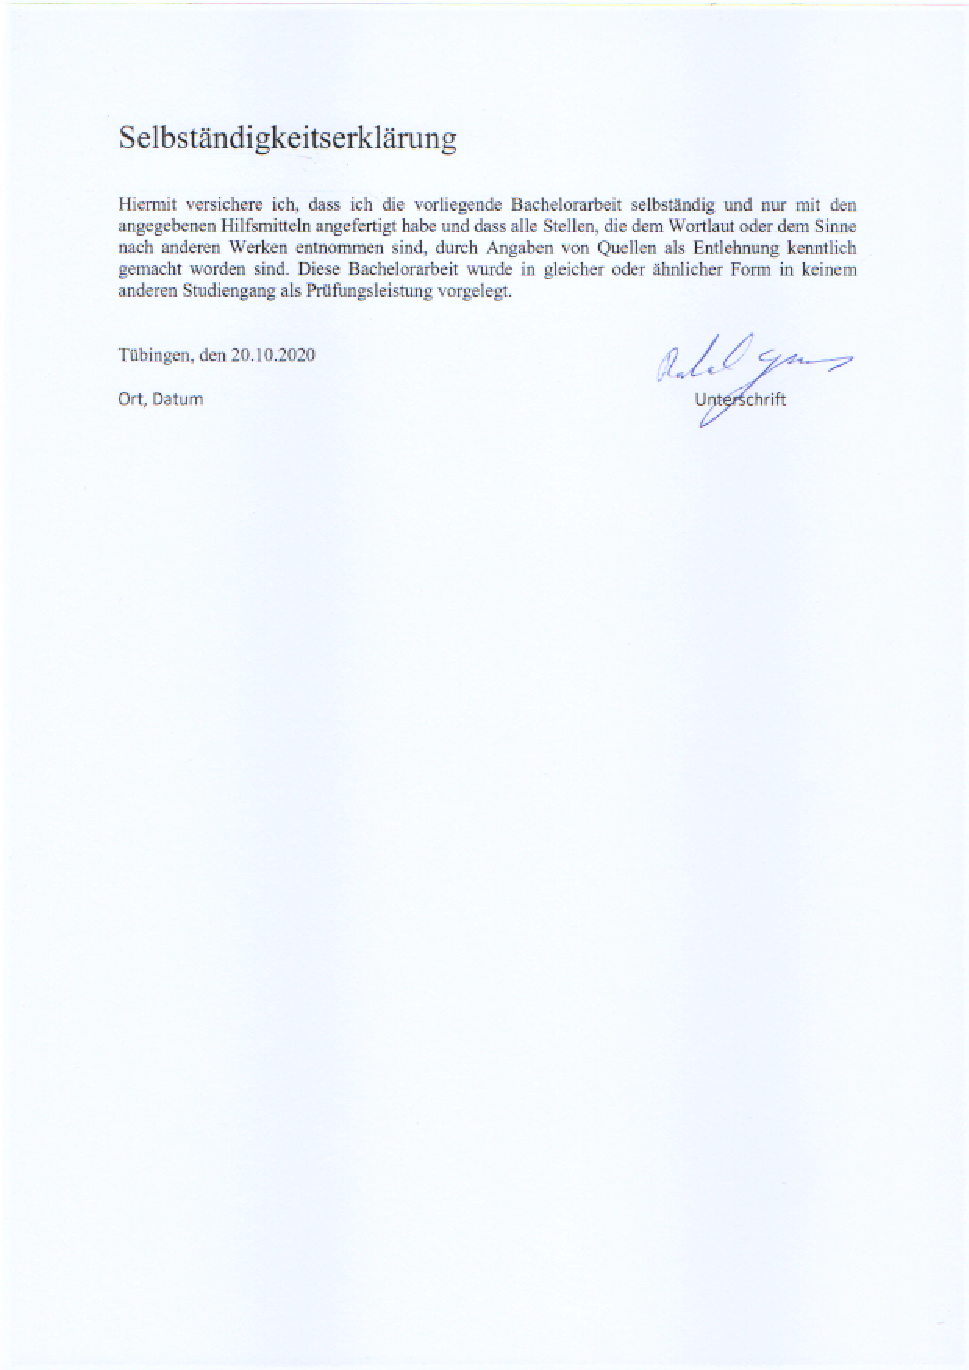
\includegraphics[page = 1]{Images/SelbstständigkeitserklärungSigned.pdf}

\end{document}